% !TEX encoding = UTF-8
% !TEX TS-program = pdflatex
% !TEX root = ../thesis.tex

%************************************************
\chapter{Hadronic Higgs Production}\label{chap:four}
%************************************************
In hadron-hadron collisions, a single Higgs boson can be produced via five main channels, listed below in descending order according to their cross sections:
\begin{enumerate}
  \item Gluon-gluon fusion ($pp \rightarrow H$),
  \item Vector-boson fusion ($pp \rightarrow qqH$),
  \item Higgs Strahlung ($pp \rightarrow WH$ or $pp \rightarrow Z H$),
  \item $t \bar{t}$ or $b \bar{b}$ associated production ($pp \rightarrow t \bar{t} H$, or $b \bar{b} H$),
  \item Single-top associated production ($pp \rightarrow t H$).
\end{enumerate}
Examples of leading-order (LO) Feynman diagrams for these channels are shown in Fig.~\ref{fig:4:channels}.
\begin{figure}[ht]
\centering
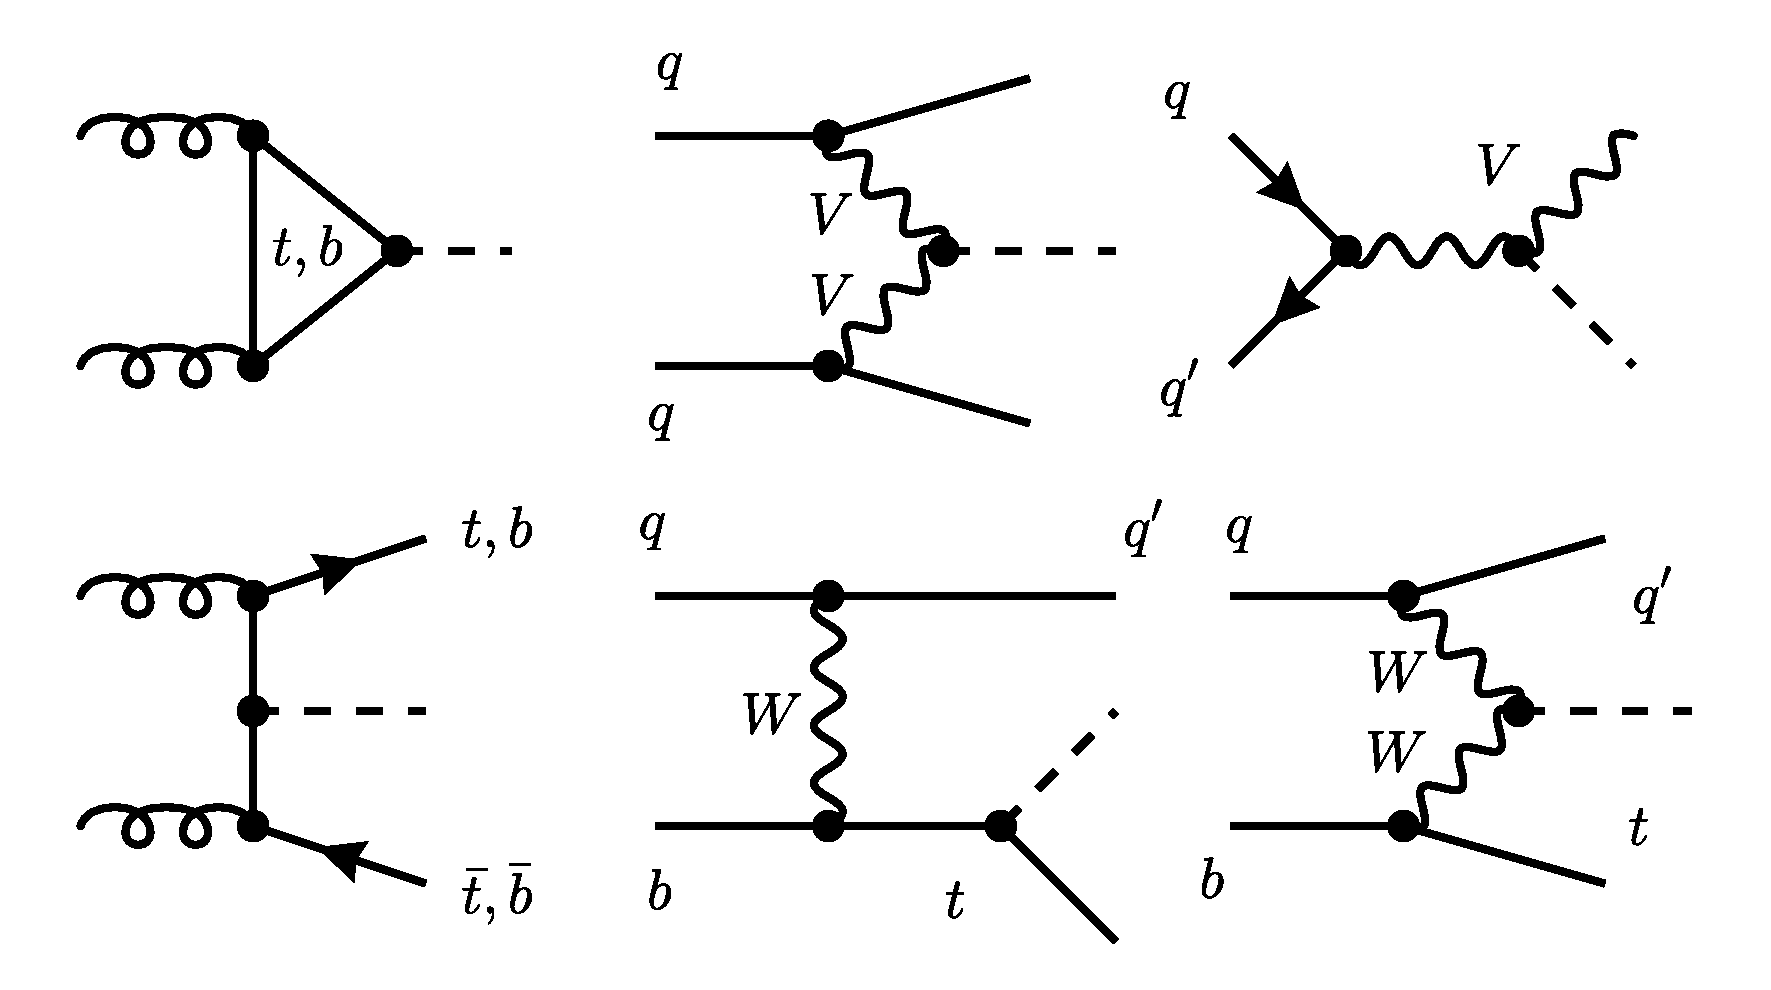
\includegraphics[scale=0.38]{Images/channels.pdf}
\caption{Example \acs{LO} Feynman diagrams for the various hadronic Higgs-production channels. From top-left to bottom-right: gluon-gluon fusion, vector-boson fusion, Higgs Strahlung, $t \bar{t}$ or $b \bar{b}$ associated production, and the last two diagrams correspond to single-top associated production. $V$ labels electroweak vector bosons, \ie\ either a $Z$ or $W$ boson. In case a fermion line is drawn without an arrow, it indicates that both fermion flows are valid. $q$ and $q^\prime$ mark massless quarks.}
\label{fig:4:channels}
\end{figure}
The cross sections for these processes span nearly three orders of magnitude, as illustrated in Fig.~\ref{fig:4:Escan}. At the lower end is single-top associated Higgs production, with a cross section of about $0.08\ \text{pb}$ at a center-of-mass energy of 13,TeV.  The next rarest channels, with cross sections of approximately $0.5\ \mathrm{pb}$, are $t \bar{t}$ and $b \bar{b}$ associated production, followed closely by the two Higgs-strahlung processes ($pp \rightarrow WH$ and $pp \rightarrow ZH$). Vector-boson fusion ranks second in magnitude, with a cross section of around 3.8~pb.
\begin{figure}[ht]
\centering
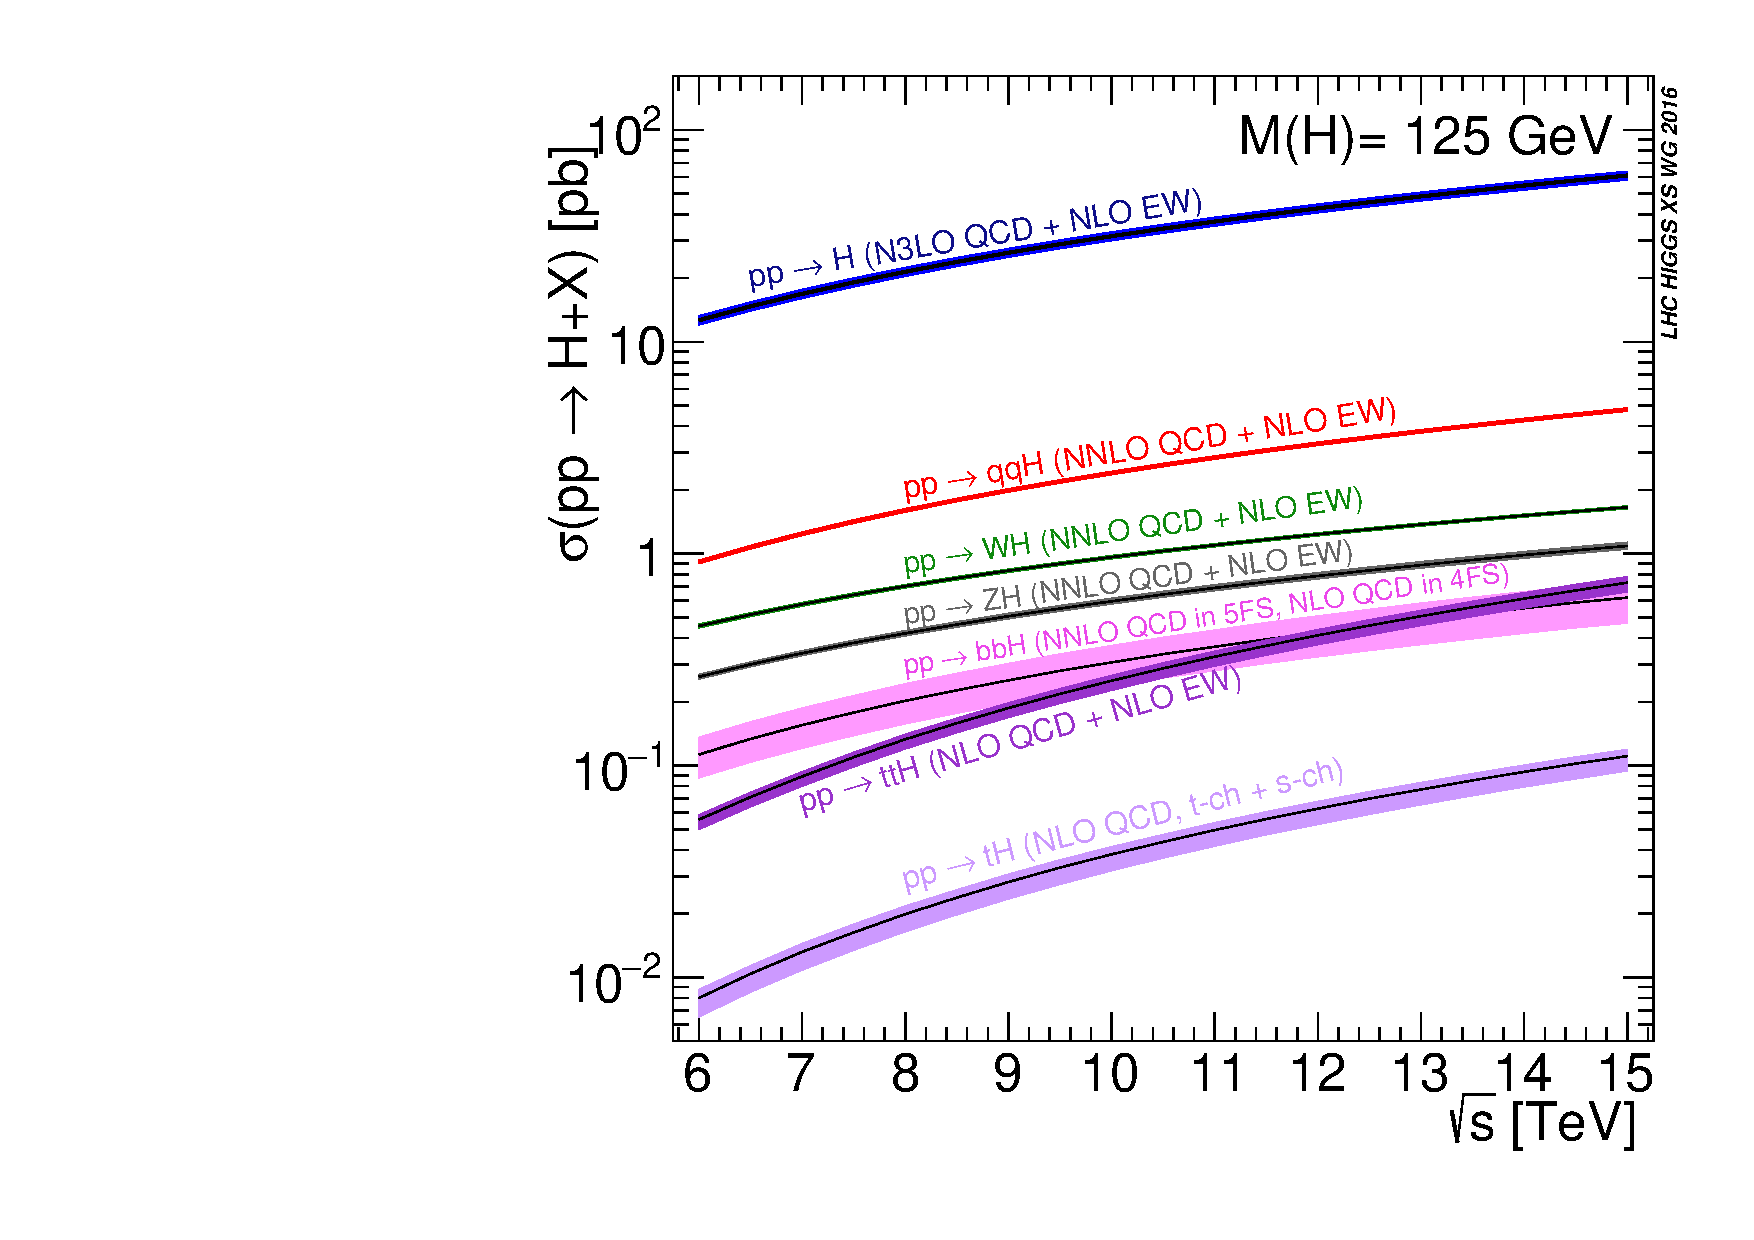
\includegraphics[scale=0.5]{Images/plot_Escan_H125_new_sqrt.pdf}
\caption{Inclusive Higgs production cross section as a function of the hadronic center-of-mass energy for various Higgs production channels. The figure was taken from Ref.~\cite{LHCHiggsCrossSectionWorkingGroup:2016ypw}.}
\label{fig:4:Escan}
\end{figure}

However, all other channels are dwarfed in comparison to the gluon-gluon-fusion channel with a cross section of approximately $46\ \mathrm{pb}$. This channel alone accounts for nearly $90\%$ of all produced Higgs bosons at the \acs{LHC}.

The relatively large production cross section of the Higgs boson has enabled experimentalists to measure it with remarkable precision. In particular, its most precise measurement (under the assumption of \acs{SM} branching ratios) is reported in Ref.~\cite{CMS:2022dwd}:
\begin{equation}
\sigma_{pp \rightarrow H}(13\ \mathrm{TeV}) = 47.1 \pm 3.8\ (\pm 8\%)\ \mathrm{pb}.
\label{eq:2:xSec_pp2H_experiment}
\end{equation}

A key theoretical tool for describing the production and decay of the Higgs is the narrow width approximation, $\Gamma_H / m_H \approx 3 \times 10^{-5} \ll 1$.
Under this approximation, the cross section for producing a Higgs boson and observing it in a particular decay mode can be factorized as
\begin{equation}
\sigma_{pp \rightarrow H \rightarrow X} = \sigma_{pp \rightarrow H} \frac{\Gamma_{H \rightarrow X}}{\Gamma_H},
\label{eq:4:narrow_width_approximation}
\end{equation}
where $\Gamma_H$ denotes the total decay width of the Higgs, and $\Gamma_{H \rightarrow X}$ is the partial decay width for the final state $X$.

Looking to the future, the planned high-luminosity phase of the \acs{LHC} (HL-LHC) offers the prospect of even more precise cross-section measurements.
As shown in Table~\ref{tab:4:HLLHC_projections}, uncertainties below 4\% are expected in some decay modes.

\begin{table}[ht!]
\centering
\begin{tabular}{lccc}
Decay Mode & CMS [\%] & ATLAS [\%] \\
\hline
$H \rightarrow \gamma \gamma$  & $\pm 2$ (stat.) $\pm 3$ (sys.)  & $\pm 2$ (stat.) $\pm 3$ (sys.) \\
$H \rightarrow Z Z^*$          & $\pm 2$ (stat.) $\pm 3$ (sys.)  & $\pm 2$ (stat.) $\pm 4$ (sys.) \\
$H \rightarrow W W^*$          & $\pm 1$ (stat.) $\pm 3$ (sys.)  & $\pm 1$ (stat.) $\pm 4$ (sys.) \\
$H \rightarrow b\bar{b}$       & $\pm 3$ (stat.) $\pm 5$ (sys.)  & $\pm 3$ (stat.) $\pm 4$ (sys.) \\
$H \rightarrow \mu^+ \mu^-$    & $\pm 9$ (stat.) $\pm 2$ (sys.)  & ${}^{+12}_{-13}$ (stat.) $\pm 3$ (sys.) \\
$H \rightarrow \tau \tau$      & $\pm 3$ (stat.) $\pm 5$ (sys.)  & $\pm 3$ (stat.) ${}^{+12}_{-10}$ (sys.) \\
\end{tabular}
\caption{Projected relative statistical and systematic uncertainties on the Higgs production cross section in the gluon-gluon-fusion channel and its subsequent decays for the high-luminosity phase of the \acs{LHC}, according to Ref.~\cite{Cepeda:2019klc}.}
\label{tab:4:HLLHC_projections}
\end{table}

Such high-precision measurements are critical for searches beyond the \acs{SM}, as experimental results must be compared closely with theoretical predictions.
Any deviation from the \acs{SM} expectation may serve as a hint of new physics, whereas agreement at this unprecedented level of accuracy places stronger constraints on extensions of the \acs{SM}.
Since the discovery of the Higgs boson in 2012~\cite{ATLAS:2012yve, CMS:2012qbp}, there has therefore been a continual drive to reduce the theoretical uncertainties of the \acs{SM} predictions. Among the various Higgs production mechanisms, the gluon-gluon-fusion channel stands out as the most precisely measured and is thus particularly important for these ongoing efforts.

In the next sections, we concentrate solely on the gluon-gluon-fusion channel.
We present explicit calculations of its cross section at leading order (\acs{LO}) and approximate next-to-leading order (\acs{NLO}), and we provide an overview of the current theoretical status along with the remaining challenges.


\section{The Leading-Order Cross Section} \label{sec:4:LO_xSec}
Having established that the gluon-gluon-fusion Higgs production cross section is central for many phenomenological applications, we now want to perform the actual \acs{LO} calculation, which was first demonstrated by Georgi et al.\ in 1978~\cite{Georgi:1977gs}. The calculation not only serves as an instructive example on cross section calculation, and thereby allows us to put our experience from Section~\ref{sec:2:cross_sections} to good use, but it already introduces many important concepts we can transfer to the \acs{NNLO} computation.

At LO, there are only two possible Feynman diagrams, depicted in Fig.~\ref{fig:4:LO}.
\begin{figure}[ht]
\centering
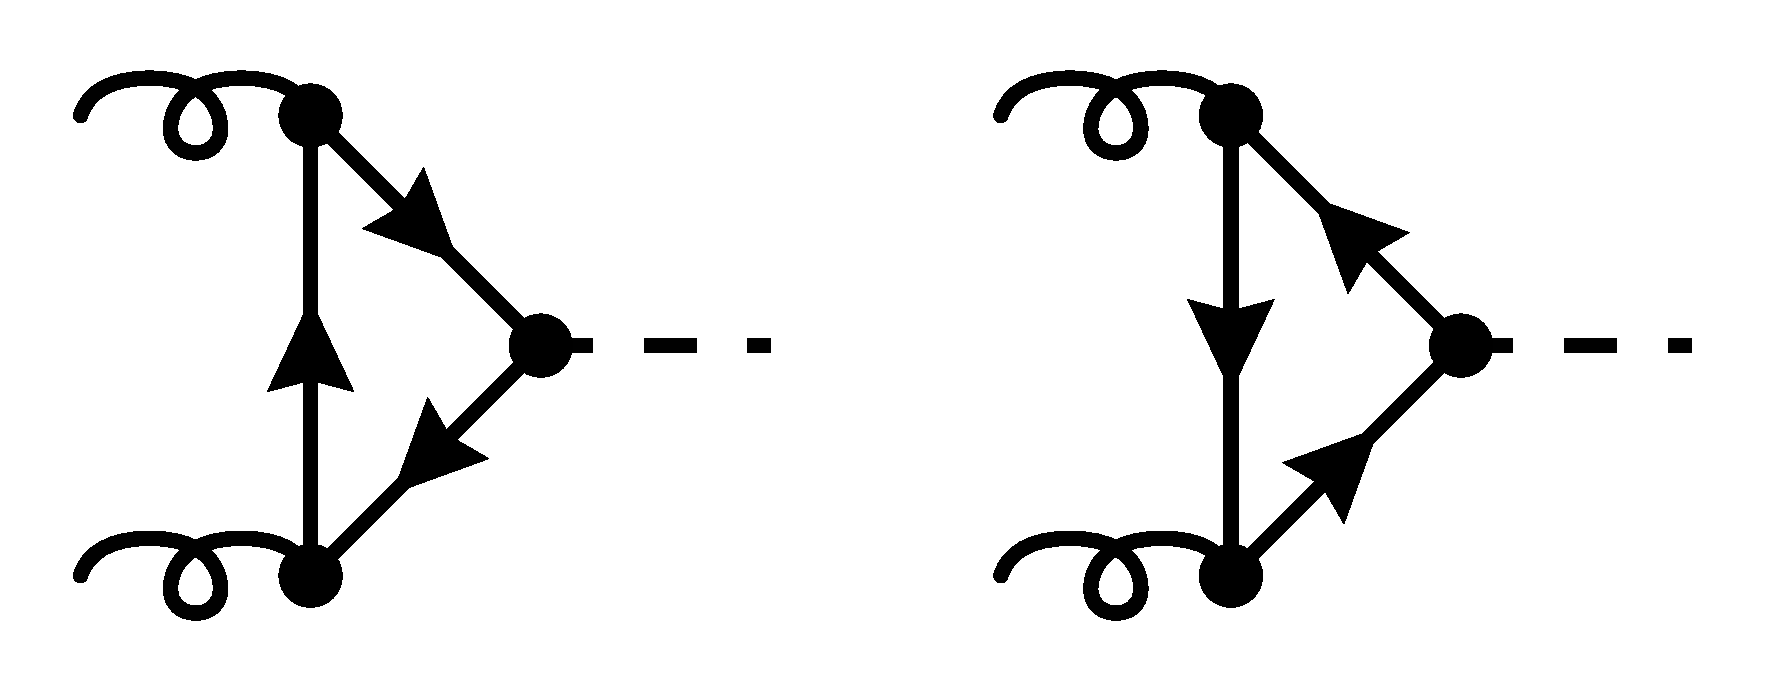
\includegraphics[scale=0.2]{Images/LO.pdf}
\caption{\acs{LO} Feynman diagrams for Higgs production in the gluon-gluon-fusion channel.}
\label{fig:4:LO}
\end{figure}
As we can see, gluon-gluon fusion is a loop induced process with two scales: the mass of the quark running in the loop $m_q$, and the Higgs mass $m_H$ which must simultaneously represent the partonic center-of-mass energy. The initial-state gluons carry the on-shell momenta $p_1$ and $p_2$. Let us then define the amputated amplitude via
\begin{equation}
i\mathcal{M} \equiv i \mathcal{M}^{\mu\nu, ab} \varepsilon_\mu^a(p_1) \varepsilon_\nu^b(p_2).
\end{equation}
With the Feynman rules presented in Appendix~\ref{app:1}, we find that the amplitude reads
\begin{equation}
\begin{split}
&i \mathcal{M}^{\mu \nu, ab} = -\int \frac{\dd^4 k}{(2\pi)^4}\, \\
&\quad \times \text{Tr}\!\left[ \frac{-i m_q}{v} \delta_{ij} \frac{i(\slashed{k} + \slashed{p}_1 + \slashed{p}_2 + m_q)}{(k + p_1 + p_2)^2 - m_q^2} (ig \gamma^\nu T^a_{ik}) \frac{i (\slashed{k} + \slashed{p}_1 + m_q)}{(k + p_1)^2 - m_q^2} (i g \gamma^\mu T^b_{kj}) \frac{i (\slashed{k} + m_q)}{k^2 - m_q^2} \right] \\
&\quad + \lbrace p_1 \longleftrightarrow p_2,  \mu \longleftrightarrow \nu, a \longleftrightarrow b \rbrace .
\label{eq:4:form_factor_amplitude}
\end{split}
\end{equation}
The extra minus sign in front of the integral stems from the closed fermion loop.

Even without performing the explicit calculation, we can already anticipate the general structure of the amplitude. Color wise, the amplitude must be proportional to $\delta^{ab}$ because it is the only available rank-two tensor. Since it is a symmetric tensor, the Lorentz structure must also be symmetric or else the amplitude would not respect \textit{Bose symmetry}. The amputated amplitude must therefore satisfy
\begin{equation}
\mathcal{M}^{\mu \nu, ab} (p_1, p_2) = \mathcal{M}^{\nu \mu, ba } (p_2, p_1).
\end{equation}
The only symmetric rank two tensors we have available are $g^{\mu\nu}$, $(p_1^\mu p_2^\nu + p_2^\mu p_1^\nu)$, $p_1^\mu p_1^\nu$, and $p_2^\mu p_2^\nu$. But since just the transverse parts give rise to physical amplitudes, the only relevant tensors are $g^{\mu \nu}$ and $p_2^\mu p_1^\nu$. Lastly, we know that the amplitude must satisfy the \textit{Ward identity}. This allows us to restrict the tensor structure even further, such that we end up with
\begin{equation}
i \mathcal{M}^{\mu \nu, ab} = i\frac{\alphas}{\pi} \frac{1}{v} \delta^{ab} \left(p_2^\mu p_1^\nu - (p_1 \cdot p_2)g^{\mu\nu} \right) \mathcal{C}(m_H, m_q).
\label{eq:4:form_factor}
\end{equation}
Notice that we have only made use of very general properties of the amplitude. This is why the decomposition in Eq.~\eqref{eq:4:form_factor} will hold at every order of $\alphas$. The function $\mathcal{C}(m_H, m_q)$ is called the \textit{Higgs-gluon form factor}. It has mass dimension 0, \ie\ its functional dependence on $m_q$ and $m_H$ must enter through a mass ratio
\begin{equation}
\mathcal{C} (m_H, m_q) = \mathcal{C}(z), \quad \text{with} \quad z \equiv \frac{m_H^2}{4 m_q^2}.
\end{equation}
The factor of $1/4$ was introduced, so that the \textit{normal threshold} is located at $z = 1$. Mathematically, this means that $z = 1$ is a solution of the \textit{Landau equations}. Physically, we can interpret the singularity as the point where we have enough energy to produce the quark pair on-shell.

The form factor can now be extracted through a simple projection
\begin{equation}
\mathcal{C}(z) = \frac{\pi v}{i \alphas} \frac{1}{N_c^2 - 1} \delta^{ab} \frac{1}{(p_1 \cdot p_2)^2 (d - 2)} \left(p_{2\,\mu} p_{1\,\nu} - (p_1 \cdot p_2) g_{\mu\nu} \right) i \mathcal{M}^{\mu \nu, ab}.
\end{equation}
Let us further define a pertubative expansion of the Higgs-gluon form factor
\begin{equation}
\mathcal{C} = \mathcal{C}^{(0)} + \frac{\alphas}{\pi} \mathcal{C}^{(1)} + \left( \frac{\alphas}{\pi} \right)^2 \mathcal{C}^{(2)} + \cdots
\label{eq:4:form_factor_expansion}
\end{equation}
If we now insert the \acs{LO} expression of Eq.~\eqref{eq:4:form_factor_amplitude} and perform some basic manipulations, we find for the leading coefficient
\begin{equation}
\begin{split}
\mathcal{C}^{(0)} (z) = T_F \frac{1}{2 - 2 \epsilon} \frac{1}{z} \int \frac{\dd^d k}{i \pi^{d/2}} \,&\frac{1}{[k^2 - m_q^2 + i0^+][(k + p_1 + p_2)^2 - m_q^2 + i0^+]} \\
& \times \left( 2 \epsilon + \frac{m_H^2}{[(k + p_1)^2 - m_q^2 + i0^+]} \left(\frac{1}{z} + \epsilon - 1 \right) \right),
\label{eq:4:C0_integral_form}
\end{split}
\end{equation}
which, after solving the appearing integrals and expanding in $\epsilon$, finally reduces to
\begin{equation}
\mathcal{C}^{(0)}(z) = T_F \frac{1}{z} \bigg \lbrace 1 - \left(1 - \frac{1}{z} \right) \left[ \frac{1}{2} \ln\! \left( \frac{\sqrt{1 - 1/z} - 1}{\sqrt{1 - 1/z} + 1} \right) \right]^2 + \BigO{\epsilon} \bigg \rbrace.
\label{eq:4:C0}
\end{equation}
The \acs{LO} Higgs-gluon form factor is plotted in Fig.~\ref{fig:4:form_factor} along with the \acs{NLO} and \acs{NNLO} corrections. As expected from the Landau equations, we pick up an imaginary part starting from the normal threshold at $z=1$.

Since the two incoming gluons are vector bosons which subsequently form a spinless final state, we would expect them to always carry opposite spins. This intuition is indeed confirmed by the tensor structure of the amplitude~\eqref{eq:4:form_factor}, as it always vanishes once contracted with two polarization vectors of the same helicity\footnote{This can be seen easily by boosting to the center-of-mass frame and using $\epsilon^\mu (-\mathbf{p}, \lambda) \propto \epsilon^\mu (\mathbf{p}, -\lambda)$.}.

\begin{figure}[ht]
\centering
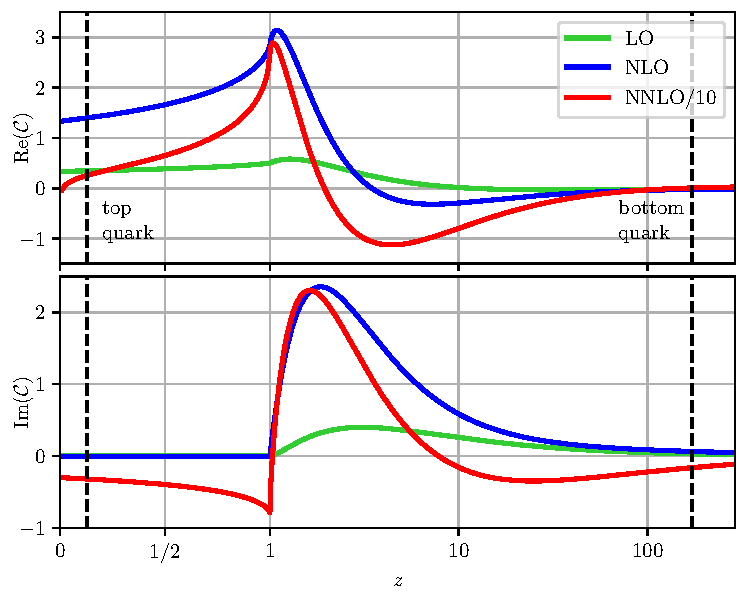
\includegraphics[width=\figurewidth]{Images/form_factor.pdf}
\caption{Real and imaginary part of the renormalized Higgs-gluon form factor at various perturbative orders. \acs{NNLO} is divided by ten for better visibility. \acs{NNLO} results also depend on the number of light-quark flavors which has been set to 5 (5\acs{FS}). The top-quark mass is renormalized in the \acs{OS} scheme. Infrared divergences are subtracted in the \MS\ scheme with the help of the $\mathbf{Z}$ operator (see \eg\ Ref.~\cite{Czakon:2014oma}). Vertical dashed lines indicate the $z$-values for the top- ($m_t$) and bottom-quark ($\overline{m}_b(m_H/2)$) masses. The renormalization scale is set to $\mu_R = -m_H$, in order to eliminate some appearing logarithms and their analytic continuation. The plot was created using the results of Ref.~\cite{Czakon:2020vql}.}
\label{fig:4:form_factor}
\end{figure}
If we expand the form factor around large quark masses, \ie\ we perform a \textit{large mass expansion} (\acs{LME}), we find that it approaches a constant
\begin{equation}
\mathcal{C}^{(0)}(z) = T_F \left( \frac{2}{3} + \frac{7}{45} z + \frac{4}{63} z^2 + \BigO{z^3} \right).
\label{eq:4:LME}
\end{equation}
We will discuss the leading term of the expansion, \ie\ the infinite mass limit, in more detail in Section~\ref{sec:4:HTL}. On the other side of the spectrum, we can see that if the mass of the Higgs is far greater than the mass of the internal quark, the form factor is approximately
\begin{equation}
\mathcal{C}^{(0)}(z) = \frac{T_F}{4z} \left[ 4 - \log^2\!\left(-4 z \right) + \frac{1}{z} \left( \log\!\left(-4 z \right) + \log^2\!\left(-4 z \right) \right) + \BigO{1/z^2} \right].
\label{eq:4:C0_HEL}
\end{equation}
This expansion is known as the \textit{high-energy limit} (\acs{HEL}) of the Higgs-gluon form factor. In this limit, the Higgs-gluon form factor is roughly proportional to the square of the mass of the quark running in the loop. One power of $m_q$ is hereby picked up from the Yukawa coupling. The other factor $m_q$ is a consequence of the scalar coupling to the Higgs. Indeed, without the quark mass, the trace in Eq.~\eqref{eq:4:form_factor_amplitude} would contain an odd number of gamma matrices and vanish consequently. Physically, we can interpret this as a helicity flip of the internal quark at the Higgs interaction vertex. And since massless \acs{QCD} conserves helicity, the other helicity flip is provided by the mass. The appearing double logarithms $\log^2 (m_q^2/m_H^2)$ originate from a soft quark exchange (For a formal proof see Ref.~\cite{Liu:2017vkm}). In fact, the quark mass acts as an infrared regulator of the integral in Eq.~\ref{eq:4:C0_integral_form}, so the appearance of these logarithms is not entirely unexpected. Numerically, these logarithms can be very large. The bottom-quark, for example, will yield a double logarithm of about $46$. \Ie, although suppressed by a factor of $m_q^2/m_H^2$, the contributions from lighter quark flavors are logarithmically enhanced and hence highly significant for precision predictions.

If we now apply Eq.~\eqref{eq:2:Xsec} and perform the phase space integration, which for a single particle is trivial because of the momentum conserving delta function, we get for the partonic cross section
\begin{equation}
\hat{\sigma}_{gg \rightarrow H}(\tau S) = \frac{\pi}{64 v^2} m_H^2 \left( \frac{\alphas}{\pi} \right)^2 |\mathcal{C}(z)|^2 \delta\! \left(\tau S - m_H^2 \right) \frac{1}{1 - \epsilon}.
\label{eq:4:ggH_cross_section}
\end{equation}
The initial state was averaged over spin and color. In conventional dimensional regularization, the gluons have $d - 2 = 2 (1 - \epsilon)$ spin degrees. Finally, after the convolution with the partonic luminosity, we arrive at the LO cross section
\begin{equation}
\sigma_{pp \rightarrow HX}^{\text{LO}}(S) = \frac{\pi}{64v^2} \left(\frac{\alphas}{\pi} \right)^2 \mathcal{L}_{gg}\!\left(\frac{m_H^2}{S} \right) |\mathcal{C}^{(0)}(z)|^2.
\end{equation}
From Fig.~\ref{fig:4:form_factor}, we can see that the top-quark exerts the largest impact on the Higgs-gluon form factor and hence the \acs{LO} hadron cross section. We can read off the partonic luminosity from Fig.~\ref{fig:2:luminosity} and find that the cross section for the top-quark induces Higgs production reads\footnote{Values of masses and coupling constants are provided in the \hyperref[chap:notation_and_conventions]{Conventions}.}
\begin{equation}
\sigma_{pp \rightarrow HX}^{\text{LO}} (t) = 16.30\ \mathrm{pb}
\end{equation}
at a hadronic center-of-mass energy of $13\ \text{TeV}$. Although expected to have a less significant impact, we can also include the effects of finite bottom-quark masses by coherently summing together the corresponding form factors. With $m_t$ and $\overline{m}_b(m_H/2)$, we find
\begin{equation}
\sigma_{pp \rightarrow HX}^{\text{LO}}(t+b) = 15.23\ \mathrm{pb},
\end{equation}
\ie\ the bottom-quark lowers the cross section by around $6.5\%$ at \acs{LO}.

To quantify the impact of the individual quarks flavors, we can decompose the cross section in terms of the respective Yukawa couplings $Y_i$:
\begin{equation}
\sigma_{pp \rightarrow HX} =  \sum_{i\le j} Y_i Y_j \sigma_{i j}.
\end{equation}
Without the inclusion of electroweak corrections this decomposition is always possible. We call
\begin{equation}
\sigma_{i \times j} = Y_i Y_j \sigma_{ij},
\end{equation}
the \textit{i-j-interference contribution} and
\begin{equation}
\sigma_{i} = Y_i^2 \sigma_{ii}
\end{equation}
the \textit{pure-i contribution} to the cross section. Both contributions are depicted at \acs{LO} in Fig.~\ref{fig:4:quark_effects}.
\begin{figure}[ht]
\centering
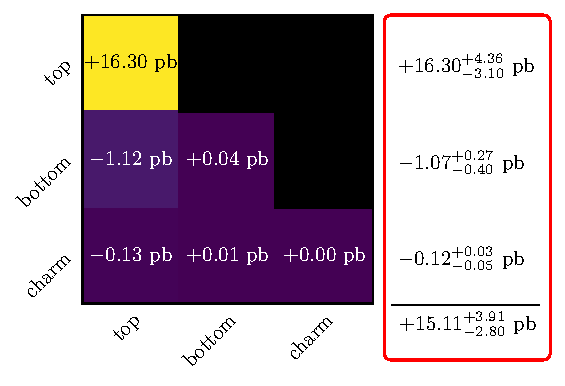
\includegraphics[scale=0.9]{Images/quark_effects_LO.pdf}
\caption{$\sigma_{i}$ (diagonals) and $\sigma_{i \times j}$ (off-diagonals) at \acs{LO} for the three heaviest quark flavors at $13\ \mathrm{TeV}$. The red box indicates the sum of each row, and hence the combined effects of each additional flavor. The computational setup is described in the \hyperref[chap:notation_and_conventions]{Conventions}. We use the on-shell mass value for the top-quark and \MS\ masses for the bottom- and charm-quark. Scale uncertainties are computed with 7-point-variation.}
\label{fig:4:quark_effects}
\end{figure}
Clearly, the dominant contribution for the lighter quark flavors comes from the interference with the top-quark. The pure-bottom contribution is already below a percent and the pure-charm quark mass effects are completely negligible. The inclusion of the charm quark lowers the total cross section by around $1\%$.


\section{The Heavy-Top Limit} \label{sec:4:HTL}
The computation of the Higgs production cross section in full \acs{QCD} is quite challenging. As we saw above, even at leading order we encounter loop integrals with two mass scales. It is therefore maybe not surprising that the first \acs{NLO} corrections to this process were actually computed in an approximation framework~\cite{Dawson:1990zj}. In the approximation, we assume that the quark, which is coupling to the Higgs is much heavier than the Higgs $z \ll 1$. That means we are only interested in the leading term of the \acs{LME}. In the \acs{SM}, the top quark is the only quark for which this approximation is applicable, which is why it is often referred to as the \textit{heavy top limit} (\acs{HTL}).

The finite distance interaction of the gluon and the Higgs will therefore shrink down to a point like vertex which we can describe with the effective Lagrangian
\begin{equation}
\mathcal{L}_{\text{HTL}}^{(0)} = \mathcal{L}_{\text{QCD}}^{(n_f - 1)} - C_1 \frac{H}{v} \frac{1}{4} G^a_{\mu \nu} G^{a\, \mu\nu}.
\label{eq:4:HTL_lagrangian}
\end{equation}
We see that the coupling constant now has mass dimension $-1$, so the theory will not be \acs{UV} renormalizable. That means that we cannot absorb all \acs{UV} divergences into multiplicative renormalization constants as we did for the \acs{SM} (see Eq.~\eqref{eq:2:renormalization}). Instead, additional independent terms must appear in our Lagrangian to cancel the arising divergences. On the other hand, as long as we focus solely on \acs{QCD} corrections and single-operator insertions, the color-singlet Higgs can be treated as a constant, and we only need to renormalize the gauge-invariant dimension-four operator
\begin{equation}
\mathcal{O}_1 \equiv -\frac{1}{4} G_{\mu\nu}^a G^{a\, \mu\nu}.
\end{equation}
To indicate the pertubative order, we gave the Lagrangian in Eq.~\eqref{eq:4:HTL_lagrangian} a superscript. The superscript $n_f - 1$ of the QCD Lagrangian specifies the number of active flavors. It was reduced by one since the heaviest quark flavor was integrated out. The constant $C_1$ is called a \textit{Wilson coefficient}, and it needs to be matched to the full theory in the infinite quark mass limit. At \acs{LO} for example, we find that the Higgs-gluon form factor in the effective theory simply reads
\begin{equation}
 \mathcal{C}^{(0)} = - \frac{\pi}{\alphas}C_1.
\end{equation}
If we compare this to the leading term of our \acs{LME}~\eqref{eq:4:LME}, we find
\begin{equation}
C_1 = -\frac{\alphas}{\pi} \frac{2}{3} T_F + \BigO{\alphas^2}.
\label{eq:4:C1_Wilson_coefficient_LO}
\end{equation}

The main benefit of the approximation lies in the reduced complexity. By integrating out the heavy quark, we have reduced a loop-induced process to a tree-level process. Moreover, the heavy-quark mass is eliminated as a scale; hence, the appearing Feynman integrals will generally be much simpler to solve.

\subsection{Renormalization of Gauge Invariant Operators}
Beyond \acs{LO}, gauge invariant operators, such as $\mathcal{O}_1$, can mix under renormalization not only with other gauge invariant operators but also, notably, with operators that are not gauge invariant. To understand this phenomenon, let us consider the following partition function:
\begin{equation}
\begin{gathered}
Z[J, K] \equiv e^{i W[J, K]} \equiv \mathcal{N} \int \mathcal{D} \Phi \, e^{i \left( S[J, K] + J \cdot \Phi + K \cdot \delta_{\text{BRS}} \Phi \right)}, \quad Z[0,0] = 1, \\
J = \left(J_\mu^a, \bar{J}^a, J^a, J_B^a, \eta, \bar{\eta}, \phi \right), \quad \Phi = \left(A^{a\, \mu}, c^a, \bar{c}^a, B^a, \bar{\psi}, \psi, \mathcal{O}_1 \right), \quad K = \left( K^a_\mu, L^a \right), \\
J \cdot \Phi \equiv \int \dd^d x\, \left[ J^{a}_\mu (x) A^{a\, \mu}(x) + \bar{J}^a(x) c^a(x) +  J^a(x)\bar{c}^a(x) + J_{B}^a(x) B^a(x) \right.  \\
\hspace{7cm} \left.+ \bar{\psi}(x) \eta(x) + \bar{\eta}(x) \psi(x) + \phi(x) \mathcal{O}_1(x) \right], \\
K \cdot \delta_{\text{BRS}} \Phi \equiv \int \dd^d x \, \left[ K^a_\mu(x) \delta_{\text{BRS}} A^{a\, \mu}(x) + L^a(x) \delta_{\text{BRS}} c^a(x) \right],
\end{gathered}
\end{equation}
where $J$ represents various sources coupled to the fields $\Phi$, and $K$ is a source specifically coupled to the \textit{Becchi-Rouet-Stora} (BRS) variation of the gauge and ghost field. The BRS transformation is defined by
\begin{equation}
\begin{gathered}
\delta_\lambda \equiv \lambda \delta_\text{BRS}, \quad \text{with } \lambda \text{ Grassmann odd, and} \\[6pt]
\delta_{\lambda} \psi = i \lambda g c^a T^a \psi, \quad \delta_\lambda A^a_\mu = \lambda (D_\mu c)^a,  \\[6pt]
\delta_\lambda c^a = - \frac{1}{2} \lambda g f^{abc} c^b c^c, \quad \delta_\lambda \bar{c}^a = \lambda B^a, \quad \delta_\lambda B^a = 0.
\end{gathered}
\end{equation}
The field $B^a$ is the \textit{Nakanishi-Lautrup} auxiliary field
\begin{equation}
B^a = -\frac{1}{\xi} \partial^\mu A^a_\mu.
\end{equation}
Its introduction causes the BRS-variation to be degree-two instead of degree-three nilpotent, \ie\ $\delta_{\text{BRS}}^2 = 0$.

As usual, we can define the effective action as the Legendre transform of the generating functional for connected Green's functions $W[J, K]$. Notice that we do not transform the BRS-variation of the fields, so the effective action is still a functional of $K$. Since the gauge-fixing Lagrangian does not receive quantum corrections, let us also define
\begin{equation}
\hat{\Gamma}[\Phi, k^a_\mu \equiv K^a_\mu + \partial_\mu \bar{c}^a, L^a] \equiv \Gamma[\Phi, k^a_\mu, L^a] - S_{\text{GF}} = \Gamma[\Phi, k^a_\mu, L^a] - \int \dd^d x\, \left(- \partial^\mu B^a A^a_\mu + \frac{\xi}{2} B^a B^a \right).
\end{equation}
Here, we also utilized that the BRS variation of the gauge field only couples to the combination $k_\mu^a = K_\mu^a + \partial \bar{c}_\mu^a$. This effective action satisfies the famous \textit{Zinn-Justin equation}~\cite{Zinn-Justin:1974ggz}
\begin{equation}
0 = \frac{\delta \hat{\Gamma}}{ \delta A^a_\mu} \cdot \frac{\delta \hat{\Gamma}}{\delta k^{a\, \mu}} + \frac{\delta \hat{\Gamma}}{\delta c^a} \cdot \frac{\delta \hat{\Gamma}}{\delta L^a}.
\label{eq:4:Zinn-Justin_equation}
\end{equation}
At \acs{NLO}, the bare effective action $\hat{\Gamma}$ can be decomposed into the Born contribution $\hat{S} = S - S_{\text{GF}}$, the finite part of the one-loop correction $\hat{\Gamma}^{1-\text{loop}}_\text{fin}$, and the divergent part of the one-loop correction $\hat{\Gamma}^{1-\text{loop}}_\text{div}$
\begin{equation}
\hat{\Gamma} = \hat{S} + \hat{\Gamma}^{1\text{-loop}}_\text{fin} + \hat{\Gamma}^{1\text{-loop}}_\text{div} + \BigO{\hbar^2}.
\end{equation}
If we insert this into the Zinn-Justin equation~\eqref{eq:4:Zinn-Justin_equation}, truncate the expression at one-loop, and only consider the divergent part we get
\begin{equation}
0 = \left[\frac{\delta \hat{S}}{\delta A^a_\mu} \cdot \frac{\delta }{\delta k^{a\, \mu}} + \frac{\delta \hat{S}}{\delta c^a} \cdot \frac{\delta}{\delta L^a} + \frac{\delta \hat{S}}{\delta k^{a\, \mu}} \cdot \frac{\delta}{ \delta A^a_\mu} + \frac{\delta \hat{S}}{\delta L^a} \cdot \frac{\delta}{\delta c^a} \right] \hat{\Gamma}^{1\text{-loop}}_\text{div} \equiv s \hat{\Gamma}^{1\text{-loop}}_\text{div}.
\label{eq:4:sGamma}
\end{equation}
Here, we also defined the \textit{linearized Slavnov operator} $s$. The operator is an extension of the BRS transformation, and is also degree-2 nilpotent. Renormalization iteratively removes the divergences at each loop order; therefore, it is straightforward to see that Eq.~\eqref{eq:4:sGamma} actually holds at every loop order. This equation tells us that although the counter terms of the effective action are not required to be gauge invariant, they must be vanishing under the action of $s$. Since counter terms are also polynomial in the external fields and have ghost number zero, one can then show~\cite{Kluberg-Stern:1974iel, Joglekar:1975nu, Henneaux:2011rma}, using \textit{Becchi-Rouet-Stora-Tyutis} (BRST) \textit{cohomology}, that the counter terms are linear combinations of BRST-exact, and gauge invariant operators
\begin{equation}
\hat{\Gamma}_{\text{ct}} = s F + \text{gauge invariant operators}.
\end{equation}

Since $s$ is nilpotent, it is easy to that the first term automatically satisfies the Zinn-Justin equation. Moreover, the equation can now be leveraged to determine a complete operator basis. Since we are not interested in Green's functions of the BRS variation of fields, we can set $K^a_\mu = L^a = 0$ for all practical purposes. We can then make the general Ansatz
\begin{equation}
\begin{split}
s F \bigg \vert_{L^a = 0, k^a_\mu = \partial_\mu \bar{c}^a} &= s \left( f[A^a_\mu, c^a, \partial_\mu \bar{c}^a] + g^a [A^a_\mu, c^a, \partial_\mu \bar{c}^a] L^a \right) \bigg \vert_{L^a = 0, k^a_\mu = \partial_\mu \bar{c}^a} \\
& = \left[\frac{\delta \hat{S}}{\delta A^a_\mu} \cdot \frac{\delta f}{\delta (\partial^\mu \bar{c}^a)} + \frac{\delta \hat{S}}{\delta (\partial^\mu \bar{c}^{a})} \cdot \frac{\delta f}{\delta A^a_\mu} + \frac{\delta \hat{S}}{\delta L^a} \cdot \frac{\delta f}{\delta c^a} + \frac{\delta \hat{S}}{\delta c^a} \cdot g^a\right]_{L^a = 0}.
\end{split}
\label{eq:4:sF}
\end{equation}
The functional derivatives can be worked out straightforwardly. The action and the Lagrangian can be decomposed into a gauge, a \textit{Faddeev-Popov}, a matter, and a source sector
\begin{equation}
\hat{S} = S_G + S_{FP} + S_M + S_S = \int \dd^d x\, \left(\mathcal{L}_G + \mathcal{L}_{FP} + \mathcal{L}_M + \mathcal{L}_S \right).
\end{equation}
The gauge-fixing term has been subtracted, so it does not appear on the right-hand side. The Lagrangians are
\begin{align*}
&\mathcal{L}_G = - \frac{1}{4} G^a_{\mu \nu} G^{a\, \mu \nu} = \frac{1}{2} A^a_\mu \left( g^{\mu \nu} \Box - \partial^\mu \partial^\nu \right) A^a_\nu - g f^{abc} \partial^\mu A^{a\, \nu} A^b_\mu A^c_\nu - \frac{1}{4} g^2 f^{abe} f^{cd e} A^{a\, \mu } A^{b \, \nu} A^c_\mu A^d_\nu, \\[8pt]
&\mathcal{L}_{FP} = \partial \bar{c} \cdot D c = \partial_\mu \bar{c}^a D^{ab\, \mu} c^b, \\[8pt]
&\mathcal{L}_M =  \sum_{i = 1}^{n_l} \bar{q}_i (i\slashed{D} - m_i) q_i, \\[8pt]
&\mathcal{L}_S = L^a \delta_{\text{BRS}} c^a  + \phi \mathcal{O}_1.
\refstepcounter{equation}
\tag{\theequation}
\end{align*}
Note that the source Lagrangian does not contain the term proportional to $K^a_\mu \delta_\text{BRS} A^{a\, \mu}$ since we defined the effective action $\hat{\Gamma}$ as a functional of $k^a_\mu$, and we set $k^a_\mu = \partial_\mu \bar{c}^a$. It is then straightforward to work out the relevant functional derivatives
\begin{align*}
\frac{\delta S_G}{\delta A^a_\mu} &= \left(g^{\mu \nu} \Box - \partial^\mu \partial^\nu \right)A^a_\nu - g f^{abc} \left(- \partial^\mu A^{b \, \nu} A^c_\nu + \partial^\nu A^{b\, \mu} A^c_\nu - \partial^\nu \left(A^b_\nu A^{c\, \mu} \right) \right) \\
&\hspace{8cm} - g^2 f^{abe} f^{cd e} A^{b \, \nu} A^{c\, \mu} A^{d}_\nu \\
&= D^{ab}_{\nu} G^{b\, \nu \mu},  \\[8pt]
\frac{\delta S_{FP}}{\delta A^a_\mu} &= - f^{abc} \partial^\mu \bar{c}^b c^c, \\[8pt]
\frac{\delta S_{M}}{\delta A^a_\mu} &= g \sum_{i = 1}^{n_l} \bar{q}_i \gamma^\mu T^a q_i,\\[8pt]
\frac{\delta S_{FP}}{\delta c^a} &= D^{ab\, \mu } \partial_\mu \bar{c}^b, \\[8pt]
\frac{\delta S_{FP}}{\delta (\partial_\mu \bar{c}^a)} &= D^{ab\, \mu} \bar{c}^b = \delta_{\text{BRS}} A^{a\, \mu}, \\[8pt]
\frac{\delta S_S}{\delta L^a} &= \delta_{\text{BRS}} c^a.
\refstepcounter{equation}
\tag{\theequation} \label{eq:4:functional_derivatives}
\end{align*}
Note that $\delta/\delta (c^a)$ and $\delta/\delta(\partial_\mu \bar{c}^a)$ are \textit{Grassmann odd}; that is, we get an additional minus sign whenever we permute the derivatives with other ghost fields. This explains, for example, the lack of a minus sign in $\delta S_{FP}/\delta c^a$. All derivatives not explicitly shown in Eq.~\eqref{eq:4:functional_derivatives} vanish either identically or after setting $L^a = 0$. These functional derivatives can now be inserted into Eq.~\eqref{eq:4:sF}, yielding
\begin{equation}
\begin{split}
sF &= \Bigg \lbrace \left[ D^{ab}_\nu G^{b\, \nu \mu} - f^{abc} \partial^\mu \bar{c}^b c^c + g \sum_{i = 1}^{n_l} \bar{q}_i \gamma^\mu T^a q_i \right] \cdot \frac{\delta}{\delta (\partial^\mu \bar{c}^a)} \\
& \hspace{4cm} + \delta_{\text{BRS}} A^{a \, \mu} \cdot \frac{\delta}{\delta A^{a\, \mu}} + \delta_{\text{BRS}} c^a \cdot \frac{\delta}{ \delta c^a} \Bigg \rbrace f  + D^{ab\, \mu} \partial_\mu \bar{c}^b \cdot g^a.
\end{split}
\end{equation}
The structure of the functionals $f[A^a_\mu, c^a, \partial_\mu \bar{c}^a]$ and $g^a [A^a_\mu, c^a, \partial_\mu \bar{c}^a]$ is almost entirely dictated by the mass dimension and the ghost number. Indeed, the effective action must be dimensionless and have vanishing ghost number. A quick inspection of the linearized Slavnov operator~\eqref{eq:4:sGamma} shows that it must satisfy
\begin{equation}
\text{dim}(s) = -3, \quad \text{and} \quad  \text{gh}(s) = 1.
\end{equation}
Consequently, the functionals $f$ and $g^a$ must fulfil
\begin{equation}
\text{dim}(f) = 3, \quad \text{gh}(f) = -1, \quad \text{dim} (g^a) = 1, \quad \text{and} \quad \text{gh} (g^a) = 1.
\end{equation}
So up to a factor, the only possible local functionals are
\begin{equation}
f[A^a_\mu, c^a, \partial_\mu \bar{c}^a](x) = \partial^\mu \bar{c}^a(x) A^a_\mu(x), \quad g^a[A^a_\mu, c^a, \partial_\mu \bar{c}^a](x) = c^a(x).
\end{equation}
In the end, we are only interested in a basis of independent operators, so we can consider $f$ and $g^a$ independently from one another. Setting $g^a$ to zero yields
\begin{equation}
\begin{split}
s F &= \left[ D^{ab}_\nu G^{b\, \nu \mu} - f^{abc} \partial^\mu \bar{c}^b c^c + g \sum_{i = 1}^{n_l} \bar{q}_i \gamma^\mu T^a q_i \right] A^{a}_\mu + \delta_{\text{BRS}} A^{a\, \mu} \partial_\mu \bar{c}^a \\
& = D^{ab}_\nu G^{b\, \nu \mu} A^a_\mu + g \sum_{i = 1}^{n_l} \bar{q}_i \slashed{A} q_i - \partial^\mu \bar{c}^a \partial_\mu c^a \\
& \equiv \mathcal{O}_4,
\end{split}
\end{equation}
where the minus sign in front of the last term of the second line stems from the anti-commutivity of the ghost fields. Similarly, setting $f$ to zero and $g^a = c^a$ yields
\begin{equation}
s F = D^{ab\, \mu} \partial_\mu \bar{c}^b c^a = (D^\mu \partial_\mu \bar{c})^a c^a = \mathcal{O}_5.
\end{equation}

In addition, the counter terms can contain additional gauge-invariant operators like
\begin{equation}
\mathcal{O}_{2} = \sum_{i = 1}^{n_l} m_i \bar{q}_i q_i.
\end{equation}
These operators are only unique up to operators vanishing by the classical equations of motions. Ergo, counter terms to $\mathcal{O}_1$ can also contain operators of the form
\begin{equation}
\mathcal{O}_3 = \sum_{i = 1} \bar{q}_i \left(\frac{i}{2} \overleftrightarrow{\slashed{D}} - m \right) q_i.
\end{equation}
Additional gauge invariant operators like $\sum_i \bar{q}_i \slashed{D} q_i$ are now no longer independent, and can be expressed in terms of linear combinations of other operators, in this case by $\mathcal{O}_2$ and $\mathcal{O}_3$. Note also that the operator $\mathcal{O}_5$ is gauge invariant, vanishes by the classical equations of motion, and---as we showed above---is BRST-exact.

The BRST-transformation generated by the linearized Slavnov-operator is a symmetry of the action. The associated conserved charge defines the physical space, \ie\ physical states are in the kernel of the charge operator. The matrix element of BRST-exact operators between physical states is thus vanishing. This is crucial, as it assures that the gauge-variant operators do not enter the computation of physical observables.

In summary, we can distinguish three types of operators: \textit{type-I operators} which are gauge invariant and have non-zero matrix elements, \textit{type-II${}_a$ operators} which are gauge invariant but give zero matrix elements due to the equation of motion, and finally \textit{type-II${}_b$ operators} which are gauge variant but BRST-exact and thus also give zero when applied to physical states.

In the present case, the complete operator basis reads
\begin{equation}
\begin{split}
\mathcal{O}_{I} &\begin{cases} &\mathcal{O}_1 = -\frac{1}{4} G^a_{\mu \nu} G^{a\, \mu\nu}, \\
&\mathcal{O}_2 = \sum_{i=1}^{n_l} m_i \bar{q}_i q_i, \end{cases} \\
\mathcal{O}_{II_a} &\begin{cases} &\mathcal{O}_3 = \sum_{i=1}^{n_l} \bar{q}_i \left( \frac{i}{2} \overleftrightarrow{\slashed{D}} - m \right) q_i, \end{cases} \\
\mathcal{O}_{II_b} &\begin{cases} &\mathcal{O}_4 = A^{a\, \mu} D^\nu G_{\nu\mu}^a + g \sum_{i=1}^{n_l} \bar{q}_i \slashed{A} q_i - \partial^\mu \bar{c}^a \partial_\mu c^a, \\
&\mathcal{O}_5 = (D_\mu \partial^\mu \bar{c})^a c^a. \end{cases}
\end{split}
\label{eq:4:operators}
\end{equation}
The operator basis is constructed only of light fields, and the light fields are defined in a decoupled theory. As previously discussed, the operator $\mathcal{O}_5$ is BRST-exact, gauge invariant, and vanishes due to the equations of motion. It thus classifies both as a type-II${}_a$ and a type-II${}_b$ operator.

Since operators of type-II cannot generate non-vanishing $S$-matrix elements through renormalization, the renormalization matrix must have the following general structure:
\begin{equation}
\begin{pmatrix}
\mathcal{O}_{I}^R \\
\mathcal{O}_{II}^R
\end{pmatrix} = \begin{pmatrix}
z^{I,I} & z^{I,II} \\
0 & z^{II,II}
\end{pmatrix} \begin{pmatrix}
\mathcal{O}_{I}^B \\
\mathcal{O}_{II}^B
\end{pmatrix}.
\label{eq:4:renormalization_matrix}
\end{equation}
Therefore, the final form of our effective Lagrangian reads
\begin{equation}
\mathcal{L}_{\text{HTL}} = \mathcal{L}_{\text{QCD}}^{(5)} + \frac{H}{v} \sum_{i=1}^5 C_i^B \mathcal{O}_i^B.
\label{eq:4:lagrangian_operator_basis}
\end{equation}
As usual, we replace the bare operators by their renormalized counterparts
\begin{equation}
C_i^B \mathcal{O}_i^B = C_i^B  Z_{ij}^{-1} \mathcal{O}_j^R.
\end{equation}
We can hence identify the renormalized Wilson coefficients as
\begin{equation}
C^R = (Z^{-1})^T C^B.
\end{equation}
Using the \acs{RGE}, we find that the \textit{anomalous dimension} matrix of the Wilson coefficients is determined through
\begin{equation}
\frac{\dd C^R}{\dd \ln \mu} = \left(Z \frac{\dd (Z^{-1})}{\dd \ln \mu} \right)^T  C^R = - \left( \frac{\dd Z}{\dd \ln \mu} Z^{-1} \right)^T C^R \equiv \gamma^T C^R .
\label{eq:4:anomalous_dimension_matrix}
\end{equation}
With the structure of the renormalization matrix~\eqref{eq:4:renormalization_matrix}, we arrive at an important conclusion: The Wilson coefficients of type-II operators cannot mix into the Wilson coefficients of type-I operators through the running in the scale. Since the type-II operators render no contribution to the scattering matrix element, we can focus our attention on the gauge invariant operators and their Wilson coefficients.

We now want to determine the $I,I$ part of the renormalization matrix $z^{I,I}$, in order to determine the running of the Wilson coefficients. Let us start by defining the generating functional
\begin{equation}
\begin{gathered}
Z[J] \equiv z[J]/z[0], \quad z[J] \equiv \int \prod_i \mathcal{D} \Phi_j\, e^{i(S + J \cdot \Phi)}, \quad S = S[A, c, \bar{c}, q, \bar{q}] \equiv \int \dd^d x\, \mathcal{L}, \\
J = \left( J^\mu, \bar{J}, J, \bar{\eta}, \eta \right), \quad \Phi = \left(\frac{1}{g} A_\mu, c, \bar{c}, q, \bar{q}\right),
\end{gathered}
\end{equation}
with the Lagrangian
\begin{equation}
\mathcal{L} \equiv -\frac{1}{4g^2} G^a_{\mu\nu} G^{a \, \mu \nu} - \frac{1}{2 \xi g^2} \left(\partial \cdot A \right)^2 + \partial^\mu \bar{c}^a (D_\mu c)^a + \bar{q} \left(\frac{i}{2} \overleftrightarrow{\slashed{D}} - m_q \right) q.
\label{eq:4:rescaled_Lagrangian}
\end{equation}
The Lagrangian is the QCD Lagrangian with only one active quark flavor and rescaled gauge fields
\begin{equation}
A^a_\mu \longrightarrow \frac{1}{g} A^a_\mu.
\end{equation}
Therefore, the covariant derivatives are now also defined in terms of the rescaled fields
\begin{equation}
D_\mu = \partial_\mu - i T_R^a A^a_\mu (x).
\end{equation}
Green's functions of the operators $\mathcal{O}_1$ and $\mathcal{O}_2$ can now be generated by applying the differential operators\footnote{We only provide the operators for the type-I operators since they are the only ones necessary for computing physical amplitudes. }
\begin{equation}
\begin{split}
&D_1 = - \frac{1}{2}g \frac{\partial}{\partial g} + \xi \frac{\partial}{\partial \xi} - \frac{1}{2} J_\mu \cdot \frac{\delta}{\delta J_\mu}, \\
&D_2 = - m_q \frac{\partial}{\partial m_q}, \\
\end{split}
\label{eq:4:differential_operators}
\end{equation}
on the partition function, that means
\begin{equation}
- i D_k z[J] = \int \prod_j \mathcal{D} \Phi_j \, \hat{\mathcal{O}}_k(0) e^{i(S + J \cdot \Phi)} \equiv z_{\mathcal{O}_k}[J].
\end{equation}
Here $\hat{\mathcal{O}}_k(0)$ denotes the Fourier transform of the operator $\mathcal{O}_k(x)$ at zero momentum. The normalization of the generating functional then properly subtracts the vacuum expectation value of the operators
\begin{equation}
-i D_k Z[J] = \frac{1}{z[0]}\int \prod_j \mathcal{D} \Phi_j \, \left(\hat{\mathcal{O}}_k(0) - \braket{\Omega | \mathcal{O}_k(0) |\Omega} \right) e^{i (S + J \cdot \Phi)} \equiv Z_{\mathcal{O}_k}.
\end{equation}
In the \MS\ scheme, the $R$-operation commutes with the differential operators in Eq.~\eqref{eq:4:differential_operators}, \ie\ the renormalized operators can be generated from the renormalized generating functional
\begin{equation}
Z_{\mathcal{O}_k^R} = -i D_k Z^R[J],
\end{equation}
which, on the other hand, is given by
\begin{equation}
\begin{gathered}
Z^R[J] = z^R[J]/z^R[0] ,\\
\quad z^R[J] = \int \prod_i \mathcal{D}\Phi_j \, e^{i(S^R + J \cdot \Phi)}, \\
S^R \equiv S[Z_3^{\prime\, 1/2} A^R, Z_3^{\prime\, -1/2} c^R, \tilde{Z}_3^{-1/2}\bar{c}^R, Z_2^{1/2} q^R, Z_2^{1/2} \bar{q}^R, Z_g g, Z_m m_q, Z_g^{-2} Z_3^\prime \xi^R].
\end{gathered}
\end{equation}
Using the chain rule, the derivatives can be reexpressed as
\begin{equation}
\begin{gathered}
-i D_k z^R[J] = \int \prod_j \mathcal{D} \Phi_j \, \left[ \hat{O}_k(0) + \sum_i (D_k \ln Z_i)  \frac{\partial S^R}{\partial \ln Z_i}\right] e^{i S^R + J \cdot \Phi}, \\
\quad \text{where}\quad  Z_i \in \big \lbrace Z_3^\prime , \tilde{Z}_3, Z_2, Z_g, Z_m \big \rbrace.
\end{gathered}
\end{equation}
With the Lagrangian of Eq.~\eqref{eq:4:rescaled_Lagrangian}, the derivatives of the action can be computed explicitly, yielding
\begin{equation}
Z_g \frac{\partial S^R}{\partial Z_g} = - 2 \hat{\mathcal{O}}_1(0), \quad \text{and} \quad Z_m \frac{\partial S^R}{\partial Z_m} = - \hat{\mathcal{O}}_2(0).
\end{equation}
We hence find that the renormalization constants are given by
\begin{equation}
\begin{alignedat}{2}
&z^{I,I}_{11} = 1 - 2 D_1 \ln Z_g = 1 + g\frac{\partial \ln Z_g}{\partial g}, \quad &&z^{I,I}_{12} = - D_1 \ln Z_m = \frac{g}{2} \frac{\partial \ln Z_m}{\partial g} \\
&z^{I,I}_{21} = 0, \quad &&z^{I,I}_{22} = 1.
\end{alignedat}
\label{eq:4:renormalization_matrix_coefficients}
\end{equation}
Here, we made use of the fact that the \MS-renormalization constants are independent of the quark mass and the gauge parameter. We can rewrite the appearing derivatives in terms of the $\beta$-function and the mass-anomalous dimension. Indeed,
\begin{equation}
\begin{gathered}
\frac{4\pi}{\alphas} \bar{\beta} \equiv \frac{\dd \ln \alphas}{\dd \ln \mu} = - \frac{\dd \ln Z_{\alphas}}{\dd \ln \mu} = - \left( \frac{\partial \ln Z_{\alphas}}{\partial \ln \alphas} \frac{\dd \ln \alphas}{\dd \ln \mu} + \frac{\partial \ln Z_{\alphas}}{\partial \ln\mu} \right) = - \left(  \frac{4 \pi}{\alphas}\bar{\beta} \frac{\partial \ln Z_{\alphas}}{\partial \ln \alphas} + 2 \epsilon \right) \\
\Rightarrow \frac{\partial \ln Z_{\alphas}}{\partial \ln \alphas} = g \frac{\partial \ln Z_g}{\partial g} = - 1 - 2 \epsilon \frac{\alphas}{4 \pi\bar{\beta}} = -1 + \frac{1}{1 - \frac{\beta}{2 \epsilon} \frac{4 \pi}{\alphas}},
\end{gathered}
\end{equation}
where, in the last step, we used the relation between the $d$- and four-dimensional $\beta$-functions
\begin{equation}
\bar{\beta} = \beta - 2 \epsilon \frac{\alphas}{4 \pi}.
\label{eq:4:d_dimensional_beta_function}
\end{equation}
Similarly, we find
\begin{equation}
\begin{gathered}
\gamma_m \equiv - \frac{\dd \ln m_q}{\dd \ln \mu} = \frac{\dd \ln Z_m}{\dd \ln \mu} = \frac{\partial \ln Z_m}{\partial \ln \alphas} \frac{\dd \ln \alphas}{\dd \ln \mu} = \frac{\partial \ln Z_m}{\partial \ln \alphas} \frac{4 \pi}{\alphas} \bar{\beta} \\
\Rightarrow \frac{\partial \ln Z_m}{ \partial \ln \alphas} = \frac{g}{2} \frac{\partial \ln Z_m}{\partial g} = \frac{\alphas}{4 \pi} \frac{1}{\bar{\beta}} \gamma_m = - \frac{\gamma_m}{2 \epsilon} \frac{1}{1 - \frac{\beta}{2 \epsilon} \frac{4 \pi}{\alphas}}
\end{gathered}
\end{equation}

Finally, we want to use the above results to calculate the anomalous dimension matrix in Eq.~\eqref{eq:4:anomalous_dimension_matrix}. The entries of the renormalization constant matrix depend only on the renormalization scale through the coupling constant, \ie\
\begin{equation}
\gamma^{I,I} = -\frac{\dd z^{I,I}}{\dd \ln \mu} (z^{I,I})^{-1} \bigg \vert_{\epsilon = 0} = -\frac{\partial z^{I,I}}{\partial \alphas} (z^{I,I})^{-1} 4 \pi \bar{\beta} \bigg \vert_{\epsilon = 0} = \frac{\partial z^{I,I\,(1)}}{\partial \alphas} 2 \alphas.
\end{equation}
Where we used that $z^{I,I}$ consists only of poles in the \MS\ scheme, and once again applied the relation between the $\beta$-functions given in Eq.~\eqref{eq:4:d_dimensional_beta_function}. $z^{I,I\, (1)}$ denotes the residue of the renormalization matrix
\begin{equation}
z^{I,I} = \mathbb{1} + \sum_{i = 1} z^{I,I\,(i)} \epsilon^{-i}.
\end{equation}
We then obtain the following form for the anomalous dimension matrix:
\begin{equation}
\gamma^{I,I} = \begin{pmatrix} 4 \pi \alphas \frac{\dd}{\dd \alphas} \left( \frac{\beta}{\alphas} \right) & - \alphas \frac{\dd \gamma_m}{\dd \alphas} \\
0 & 0 \end{pmatrix}.
\end{equation}
The structure of this matrix reveals that the $C_1$ Wilson coefficient, which is the relevant coefficient for the  \acs{HTL}, is completely independent of the other Wilson coefficients. The \acs{RGE} for the Wilson coefficient~\eqref{eq:4:anomalous_dimension_matrix} can now be written as:
\begin{equation}
\frac{\partial C_1}{\partial \alphas} 4 \pi \beta + \frac{\partial C_1}{\partial \ln \mu} = 4 \pi \alphas \frac{\dd }{\dd \alphas} \left(\frac{\beta}{\alphas} \right) C_1.
\label{eq:4:RGE_of_C1}
\end{equation}
The $\beta$-function has the general expansion
\begin{equation}
\beta = \left(\frac{\alphas}{4 \pi} \right)^2 \sum_{i = 0} \beta_i \left(\frac{\alphas}{4 \pi} \right)^i.
\end{equation}
For example, at one-, and two-loop level, it can be shown~\cite{Gross:1973id, Politzer:1973fx, tHooft:1972ikm, Caswell:1974gg, Jones:1974mm, Egorian:1978zx}
\begin{equation}
\begin{split}
&\beta_0 = -\frac{11}{3} C_A + \frac{4}{3} T_F n_f, \\
&\beta_1 = -\frac{34}{3} C_A^2 + \frac{20}{3} C_A T_F n_f + 4 C_F T_F n_f.
\end{split}
\label{eq:4:beta0_and_beta1}
\end{equation}
We can solve the partial differential equation in Eq.~\eqref{eq:4:RGE_of_C1} perturbatively by proposing the Ansatz
\begin{equation}
\begin{split}
C_1 =  &\ \frac{\alphas}{4 \pi} C_1^{(0,0)} + \left(\frac{\alphas}{4 \pi} \right)^2 \left(C_1^{(1,0)} + C_1^{(1, 1)} \ln \frac{\mu}{\mu_0} \right) \\
&+ \left(\frac{\alphas}{4 \pi} \right)^3 \left(C_1^{(2, 0)} + C_1^{(2, 1)} \ln \frac{\mu}{\mu_0} + C_1^{(2, 2)} \ln^2 \frac{\mu}{\mu_0} \right) + \cdots.
\end{split}
\end{equation}
The coefficients without logarithms, $C_1^{(i, 0)}$, mark the initial conditions; they need to be matched to the full theory in the infinite mass limit. The coefficients of the logarithms, on the other hand, can be determined through a comparison of coefficients; they read:
\begin{equation}
\begin{gathered}
C_1^{(1,1)} = 0, \\
C_1^{(2,1)} = C_1^{(0,0)} \beta_1 - C_1^{(1, 0)} \beta_0, \quad C_1^{(2, 2)} = 0, \\
C_1^{(3,1)} = 2 C_1^{(0,0)} \beta_2 - 2 C_1^{(2,0)} \beta_0, \quad C_1^{(3,2)} = \beta_0^2 C_1^{(1,0)} - \beta_0 \beta_1 C_1^{(0,0)}, \quad C_1^{(3, 3)} = 0.
\end{gathered}
\end{equation}
It is clear from the structure of the differential equation that all coefficients $C_1^{(i, i)}$ are indeed zero except for $C_1^{(0,0)}$.

\subsection{Matching of Wilson Coefficients} \label{subsec:4:matching_of_wilson_coefficients}
By expanding the Higgs-gluon form factor for large quark masses, we were able to determine the \acs{LO} Wilson coefficient (see Eq.~\eqref{eq:4:C1_Wilson_coefficient_LO}). Of course, if we needed the full Higgs-gluon form factor to determine the Wilson coefficient, the \acs{HTL} would be of little use, as it would not provide any simplifications. Fortunately, the large quark mass limit can already be used at the integrand level using the large mass expansion, thus tremendously simplifying the computation of the amplitudes.

Alternatively, one may find the matching coefficients by means of a \textit{low-energy theorem}~\cite{Kniehl:1994ju, Kniehl:1995tn, Chetyrkin:1997un}, which states:
\begin{equation}
-i G_{\mathcal{O}_1,\dots,\mathcal{O}_n, \bar{q}_i q_i}^B(p_1, \ldots, p_{n - 1}, 0)  = \frac{\partial}{\partial m_i^B} G_{\mathcal{O}_1,\dots , \mathcal{O}_n}^B (p_1, \ldots, p_{n - 1}).
\label{eq:4:LET}
\end{equation}
Here, $\mathcal{O}_1, \ldots , \mathcal{O}_n$ are local operators and $G_{\mathcal{O}_1,\dots} $ denotes the momentum space representation of the corresponding Green's functions
\begin{equation}
\begin{split}
& \int \left(\prod_{i = 1}^n \dd^d x_i \, e^{i p_i\cdot x_i} \right) \braket{\Omega | T \left[ \mathcal{O}_1^B(x_1) \dots \mathcal{O}_n^B(x_n) \right] | \Omega}  \\
& \hspace{3cm} \equiv (2 \pi)^d \delta^{(d)}\! \left(\sum_{i = 1}^n p_i \right) G_{\mathcal{O}_1,\dots, \mathcal{O}_n}^B(p_1, \ldots , p_{n - 1}) .
\end{split}
\end{equation}
$\ket{\Omega}$ hereby denotes the vacuum state of the interacting theory and $T$ is the \textit{time ordering operator}. The theorem relates the mass derivative of a Green's function to a Green's function of the same operators but with the insertion of $\bar{q}_i q_i$ at zero momentum.

The theorem follows upon application of the \textit{Gell-Mann--Low formula}
\begin{equation}
\begin{split}
&\frac{\partial}{\partial m_i^B} \braket{\Omega | T \left[ \mathcal{O}_1^B(x_1) \dots \mathcal{O}_n^B(x_n) \right] | \Omega}  = \mathcal{N}  \langle 0 | T \left[ \mathcal{O}_{1,I}^B(x_1) \dots \mathcal{O}_{n,I}^B(x_n) \right. \\
&\hspace{3cm} \left.  \times (-i) \int \dd^d x\, \left( 1 + \frac{H_I^B(x)}{v} \right) \bar{q}_{i}^B(x) q_i^B(x) \exp\!\left(-i \int \dd^d z \, \mathcal{H}_{\text{int}, I}^B(z) \right) \right] | 0 \rangle .
\end{split}
\label{eq:4:Gell-Mann-Low}
\end{equation}
The subscript $I$ indicates interaction picture fields, $\ket{0}$ is the vacuum state, now of the free theory, and $\mathcal{H}_{\text{int}}$ is the interaction part of the \textit{Hamiltonian}. The normalization factor $\mathcal{N}$ is defined as
\begin{equation}
\mathcal{N}^{-1} = \braket{0| T \exp\!\left(-i \int \dd^d z \, \mathcal{H}_{\text{int}, I}^B (z) \right) |0},
\end{equation}
and it cancels the disconnected contributions of the numerator on the right-hand side of Eq.~\eqref{eq:4:Gell-Mann-Low}. In the absence of electroweak corrections, we can omit the field of the Higgs\footnote{Not to be confused with the Higgs field.} in the integral of Eq.~\eqref{eq:4:Gell-Mann-Low}. This also implies that none of the operators $\mathcal{O}_1, \ldots , \mathcal{O}_n$, contain any electroweak fields, which would cause \textit{Wick contractions} with the Higgs.
After switching to momentum space, we then immediately arrive at Eq.~\eqref{eq:4:LET}.

Since the proof relied on relations at the level of the Lagrangian, the statement is true only for bare amplitudes and Green's functions beyond \acs{LO}. It can be straightforwardly generalized to include an arbitrary number of massive particles by simply summing over all massive particles. Lastly, we note that the differential operator does not act on any masses present within the operators themselves.

We can now apply the low-energy theorem to the gluon self-energy. Let us first consider the \textit{amputated} Green's function of two gluons with the insertion of the composite operator $\mathcal{O}_h = \bar{h}^B h^B$, where $h$ indicates a heavy quark field. In momentum space, it reads
\begin{equation}
\begin{split}
G_{A,A,\mathcal{O}_h}^{B,ab\,\mu\nu} (p, 0) \Big \vert_{\text{amp.}} &=  \int \dd^d x\, \dd^d y\, e^{ip \cdot (x - y)} \braket{\Omega|T\left[ A^{B,a\mu}(x) A^{B, b\nu}(y) \mathcal{O}_h(0) \right]|\Omega} \Big \vert_{\text{amp.}} \\
& \equiv \delta^{ab} \left[-g^{\mu\nu} p^2 G_{A,A,\mathcal{O}_h}^B(p^2)\Big \vert_{\text{amp.}} + \text{terms proportional to } p^\mu p^\nu \right],
\end{split}
\end{equation}
where $T$ denotes the time ordering operator and $p$ is the momentum along the gluon line. As discussed in detail above, in the limit of an infinite quark mass $m_h^B \rightarrow \infty$, the operator $\bar{h}^B h^B$ can be expressed as a linear combination of the operators $\mathcal{O}_1,\ldots , \mathcal{O}_5$
\begin{equation}
\begin{split}
&G_{A,A,\mathcal{O}_h}^{B,ab\, \mu\nu} (p, 0) \Big \vert_{\text{amp.}} \simeq \\
&\quad - \int \dd^d x\, \dd^d y\, e^{ip\cdot (x - y)} \braket{\Omega| T \left[ A^{B,a\mu}(x) A^{B, b \nu}(y) \frac{1}{m_h^B} \sum_{i=1}^5 C_i^B \mathcal{O}_i^B(0) \right]|\Omega} \Big \vert_{\text{amp.}}.
\end{split}
\end{equation}
The $\simeq$ symbol indicates that the relation holds only up to power corrections of order $1/{m_h^B}^2$.

As noted earlier, the operators $\mathcal{O}_1, \ldots , \mathcal{O}_5$ are defined in a decoupled theory in which the heavy quark has been integrated out. In the \MS\ scheme, the \textit{Appelquist-Carazzone decoupling theorem}~\cite{Appelquist:1974tg} does not hold in its na\"ive sense, \ie\ heavy degrees of freedom, do not decouple at low energy. The standard method to circumvent this issue is by introducing decoupling constants. These relate quantities in the decoupled theory (denoted with a superscript $(n_l)$) with the full high energy theory:
\begin{equation}
\begin{gathered}
g^{B, (n_l)} = \zeta_g^B g^{B}, \quad m_i^{B, (n_l)} = \zeta_{m_i}^B m_i^B, \quad \xi^{B,(n_l)} - 1 = \zeta_3^{B} (\xi^{B} - 1), \\
q_i^{B,(n_l)} = \sqrt{\zeta_2^B} q_i^{B}, \quad A_\mu^{B,(n_l),a} = \sqrt{\zeta_3^B} A^{B, a}_\mu, \quad c^{B,(n_l),a} = \sqrt{\tilde{\zeta}_3^B} c^{B,a}.
\end{gathered}
\label{eq:4:decoupling}
\end{equation}
The purpose of the decoupling constants is to absorb any residual logarithmic dependence on the decoupled fields. The decoupling relations therefore only hold up to power corrections of $1/m_h^2$. The decoupling constants are functions of $g^B, m_i^B$ and the scale $\mu$, but the function arguments are left implicit. The amputated Green's function then becomes\footnote{Note that the \textbf{amputated} Green's function scales with the inverse of the fields.}
\begin{equation}
\begin{split}
&G_{A,A,\mathcal{O}_h}^{B,ab\, \mu\nu} (p, 0) \Big \vert_{\text{amp.}} \simeq \\
&\quad- \zeta_3^B \int \dd^d x\, \dd^d y\, e^{ip\cdot (x - y)} \braket{\Omega| T \left[ A^{B,(n_l),a\mu}(x) A^{B, (n_l), b \nu}(y) \frac{1}{m_h^B} \sum_{i=1}^5 C_i^B \mathcal{O}_i^B(0) \right] |\Omega} \Big \vert_{\text{amp.}} \\
\end{split}
\end{equation}
At \acs{LO} in $\alphas$, we will have only contributions from the operators $\mathcal{O}_1$ and $\mathcal{O}_4$, as all other operators would yield disconnected contributions
\begin{equation}
\begin{split}
&G_{A,A,\mathcal{O}_h}^{B,ab\, \mu\nu} (p, 0) \Big \vert_{\text{amp.}}  \simeq \\
&\quad -\frac{1}{m_h^B}\delta^{ab} \left(-g^{\mu \nu} p^2 \zeta_3^B \left( C_1^B + 2 C_4^B \right) + \BigO{\alphas} \right) + \text{terms proportional to } p^\mu p^\nu .
\end{split}
\end{equation}
We now set the mass of light quarks in the \acs{QCD} Lagrangian to zero; however, their masses as defined in Eq.~\eqref{eq:4:operators} may still be non-vanishing. In the limit of vanishing gluon momentum $p \rightarrow 0$, the coefficient of the transverse part does not receive any $\alphas$-corrections in \acs{DR} since all Feynman integrals involved are necessarily scaleless\footnote{Typically, limits like $p \rightarrow 0$ do not permute with the integrals. However, as we are working in \acs{DR}, we can always find a dimension $d$ for which the appearing integral is vanishing in the limit $p \rightarrow 0$, as it can only depend on $p^2$. Indeed, any such integral with positive mass dimension will necessarily vanish in this limit. We can then argue based on the identify theorem that the integral must in fact be vanishing for all $d$.}. We have thus shown the all-orders result:
\begin{equation}
\begin{gathered}
G_{A,A,\mathcal{O}_h}^B(0, 0)  \Big \vert_{\text{amp.}} \simeq -  \frac{1}{m_h^B} \zeta_3^B \left(C_1^B + 2 C_4^B \right). \\
\end{gathered}
\end{equation}
By applying the LSZ reduction formula, we can rewrite the amputated Green's functions in terms of connected ones. The operator $\mathcal{O}_h$ is hereby irrelevant as it is not considered to be external. Eq.~\eqref{eq:4:LET} thus holds for regular, connected and \acs{1PI} Green's functions. Application of Eq.~\eqref{eq:4:LET} then yields
\begin{equation}
\left(C_1^B + 2 C_4^B \right) = \frac{\partial \ln \zeta_3^B}{\partial \ln m_h^B}.
\label{eq:4:gluon_decoupling_relation}
\end{equation}

We can repeat the same analysis for $G_{\bar{c}, c, \mathcal{O}_h}(p, 0)$ and $G_{\bar{c}, c, g, \mathcal{O}_h} (p, p, 0)$; in the limit as $p \rightarrow 0$, we obtain
\begin{equation}
\begin{split}
&\left( - C_4^B - C_5^B \right) = \frac{\partial \ln \tilde{\zeta}_3^B}{\partial \ln m_h^B} \\
&\left( - C_5^B \right) = \frac{\partial}{\partial \ln m_h^B} \ln\!\left(\tilde{\zeta}_3^B \sqrt{\zeta_3^B} \zeta_g^B \right)
\end{split}
\label{eq:4:ghost_and_vertex_decoupling_relation}
\end{equation}
Eq.~\eqref{eq:4:gluon_decoupling_relation} and\ \eqref{eq:4:ghost_and_vertex_decoupling_relation} form a linear system of equations that we can solve for the Wilson coefficients. The solution for the physical Wilson coefficient reads
\begin{equation}
C_1^B = - \frac{\partial \ln {\zeta_g^{B}}^2}{\partial \ln m_h^B}.
\label{eq:4:C1_Wilson_coefficient}
\end{equation}
In the \MS\ scheme, the renormalization constant of the heavy-quark mass is independent of the mass, \ie
\begin{equation}
\frac{\partial}{\partial \ln m_h^B} = \frac{\partial}{\partial \ln m_h}.
\end{equation}
With the renormalization matrix in Eq.~\eqref{eq:4:renormalization_matrix_coefficients} we can then find the renormalized version of Eq.~\eqref{eq:4:C1_Wilson_coefficient}
\begin{equation}
C_1 = - \frac{\partial \ln \zeta_g^2}{\partial \ln m_h}.
\end{equation}

The decoupling constants are known at two-, three-\cite{Chetyrkin:1997sg}, and four-loop~\cite{Schroder:2005hy, Chetyrkin:2005ia} order. Note that we only require the logarithmic dependence of decoupling constants to obtain the Wilson coefficients. The logarithmic structure on the other hand may be reconstructed from lower order terms in combination with the $\beta$-function and the mass anomalous dimension~\cite{Chetyrkin:1997un}. The four-loop decoupling constant is therefore sufficient to match the Wilson coefficient up to N${}^4$LO. Here we present only the Wilson coefficient up to N${}^3$LO, as it is the highest order for which full cross section calculations are available at present:
\begin{equation}
\begin{split}
&C_1^{(0,0)} = -\frac{4}{3}, \\
&C_1^{(1,0)} = -\frac{44}{3}, \\
&C_1^{(2,0)} = -\frac{5554}{27}  + \frac{76}{3} \ln\!\left(\frac{m_h^2}{\mu^2} \right) +  n_l \left[\frac{134}{9} + \frac{64}{9} \ln\!\left(\frac{m_h^2}{\mu^2} \right) \right], \\
&C_1^{(3,0)} = \frac{2892659}{486} - \frac{897943}{108} \zeta (3) + \frac{13864}{27} \ln\!\left(\frac{m_h^2}{\mu^2} \right) - \frac{836}{3} \ln^2\!\left(\frac{m_h^2}{\mu^2} \right) - \frac{64}{81} \ln^3\!\left(\frac{m_h^2}{\mu^2} \right) \\
& \hspace{1cm} + n_l \left[-\frac{40291}{243} + \frac{110779}{162} \zeta (3) + \frac{7040}{81} \ln\!\left(\frac{m_h^2}{\mu^2} \right) - \frac{184}{3} \ln^2\!\left(\frac{m_h^2}{\mu^2} \right) \right]    \\
& \hspace{1cm} + n_l^2 \left[ \frac{13730}{729} + \frac{308}{81} \ln\!\left(\frac{m_h^2}{\mu^2} \right) + \frac{128}{27} \ln^2\!\left(\frac{m_h^2}{\mu^2} \right) \right].
\end{split}
\end{equation}
Notice that the decoupling constant $\zeta_g$ is a function of $\alphas^{(n_l + 1)}$, \ie\ we must recursively apply the decoupling relations~\eqref{eq:4:decoupling} to express everything in terms of decoupled quantities. The heavy mass $m_h$ is the \MS\ mass.



\subsection{Higher-Order Corrections}
With the effective theory matched, we are ready to discuss higher order corrections to the Higgs production cross section. In the \acs{HTL}, the cross section has been computed up to N${}^3$LO in the literature~\cite{Dawson:1990zj, Harlander:2002wh, Anastasiou:2002yz, Anastasiou:2016cez}. Here, we will briefly recapitulate the \acs{NLO} calculation, as it nicely illustrates the methods introduced in Section~\ref{sec:2:cross_sections}, and already allows for some important observations.

We start with the computation of the hard scattering amplitudes. At \acs{NLO}, we require the one-loop Higgs-gluon form factor, and the tree-level amplitudes for $q \bar{q} \rightarrow H g$, $q g \rightarrow H q$, and $g g \rightarrow H g$.

The careful reader might wonder why we do not need to compute the $q \bar{q} \rightarrow H$ amplitude. The reason is that these amplitudes will be zero at all orders. Indeed, the corresponding amplitude takes on a form
\begin{equation}
\mathcal{M}_{q \bar{q} \rightarrow H} = i \frac{\alphas}{\pi} \bar{v}(p_2) \left[ \cdots \right] u(p_1) \delta_{c_1 c_2} \frac{1}{v} \mathcal{C}_{q \bar{q} H},
\label{eq:4:quark_form_factor}
\end{equation}
where the dots indicate an a priori unknown number of $\gamma$-matrices. However, since there is no external vector field, the $\gamma$-matrices must be contracted. The only available objects to contract a $\gamma$-matrix with are either other $\gamma$-matrices, or the momenta $p_1$ or $p_2$. Contractions among $\gamma$-matrices can always be simplified by applying the anti-commutation relations provided by the Clifford algebra of the $\gamma$-matrices. Afterwards, we are left only with contractions involving $p_1$ and $p_2$. These, on the other hand, vanish in Eq.~\eqref{eq:4:quark_form_factor} due to the equation of motion.

The virtual contributions to the cross sections result from evaluating the Feynman diagrams in Fig.~\ref{fig:4:ggH}. The result is the NLO correction to the Higgs-gluon form factor in the \acs{HTL} and reads
\begin{equation}
\mathcal{C}(0) = \frac{1}{3} \bigg \lbrace 1 + \frac{\alphas}{\pi} \left(- \frac{m_H^2 + 0^+}{\mu^2} \right)^{-\epsilon} \left(-\frac{3}{2} \frac{1}{\epsilon^2} + \frac{11}{4} + \frac{\pi^2}{8} \right) \bigg \rbrace .
\label{eq:4:HTL_formfactor}
\end{equation}
\begin{figure}[ht]
\centering
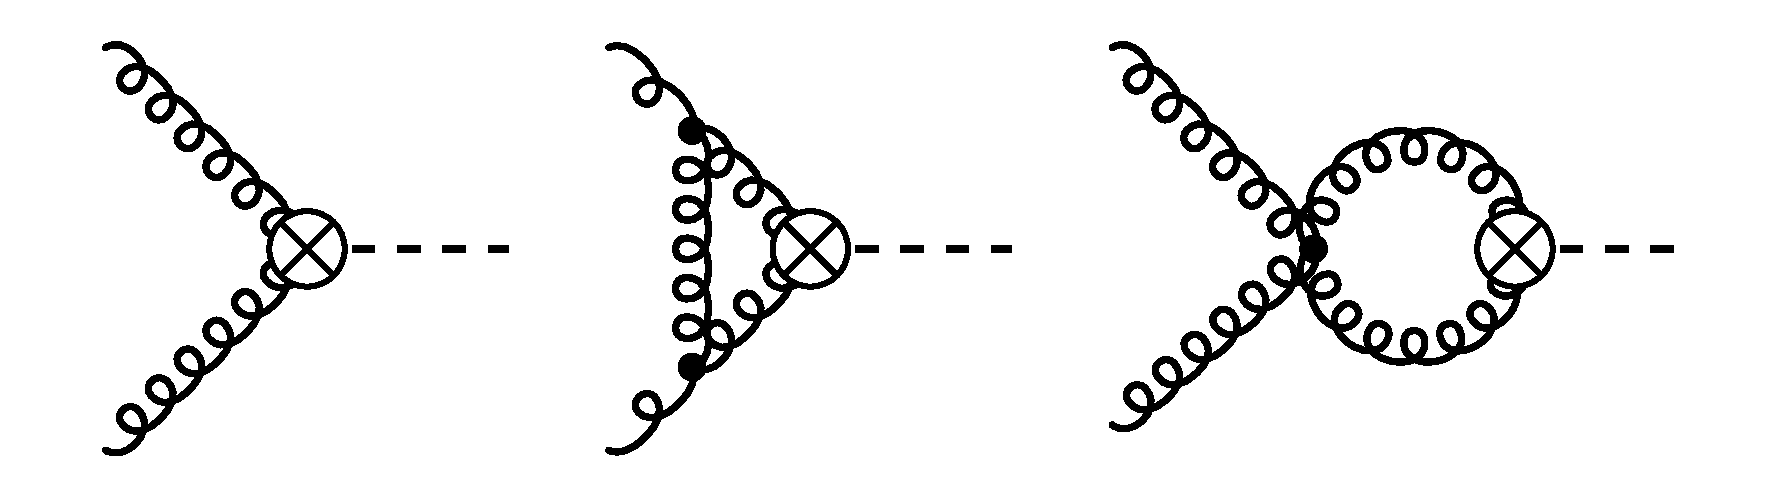
\includegraphics[scale=0.3]{Images/NLO_Feynman_diagrams/ggH.pdf}
\caption{One-loop corrections to the Higgs-gluon form factor. The first diagram contributes through the NLO Wilson coefficient.}
\label{fig:4:ggH}
\end{figure}
Using Eq.~\eqref{eq:4:ggH_cross_section} for the partonic $gg \rightarrow H$ cross section, we then find
\begin{equation}
\begin{split}
&\hat{\sigma}_{gg \rightarrow H} = \frac{\pi}{576 v^2} \xi  \left(\frac{\alphas}{\pi} \right)^2 \delta(1 - \xi) \\
&\qquad \times \left[ \left( 1 + \epsilon + \BigO{\epsilon^2} \right) + \frac{\alphas}{\pi} \left(\frac{m_H^2}{\mu^2} \right)^{-\epsilon} \left(-\frac{3}{\epsilon^2} - \frac{3}{\epsilon} + \frac{5}{2} + \frac{7 \pi^2}{4} + \BigO{\epsilon} \right) + \BigO{\alphas^2} \right]
\label{eq:4:ggH_VV}
\end{split}
\end{equation}
where we defined $\xi$ as the square of the Higgs mass over the partonic center-of-mass energy
\begin{equation}
  \xi = \frac{m_H^2}{s} = \frac{m_H^2}{\tau S}.
\end{equation}
\begin{figure}
  \centering
  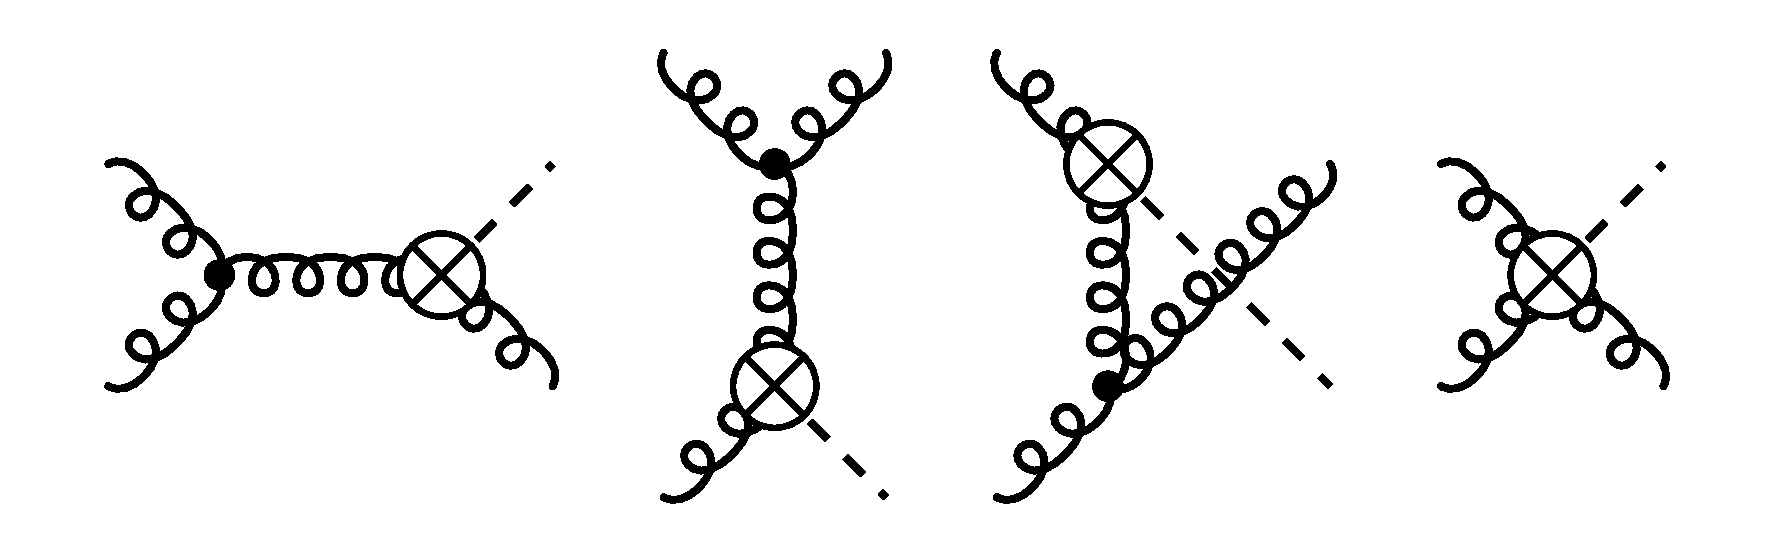
\includegraphics[scale=0.3]{Images/NLO_Feynman_diagrams/ggHg.pdf}
  \caption{Feynman diagrams for the real radiation corrections in the gluon-gluon channel.}
  \label{fig:4:ggHg}
\end{figure}

As expected, the \acs{NLO} partonic cross section is not finite by itself because the \acs{IR} divergences only cancel in inclusive observables. Therefore, we must also compute the real radiation corrections as well as the contributions from collinear renormalization. For the former, we evaluate the diagrams shown in Fig.~\ref{fig:4:ggHg} and obtain the averaged squared amplitude
\begin{equation}
\overline{|\mathcal{M}_{gg \rightarrow H g}|^2} = \frac{1}{N_A^2 4 (1 - \epsilon)^2} \frac{\alphas^3}{v^2} \left(\frac{32}{3 \pi} \right) \left[ (1 - 2 \epsilon) \frac{m_H^8 + s^4 + t^4 + u^4}{stu} + \frac{\epsilon}{2} \frac{\left(m_H^4 + s^2 + t^2 + u^2 \right)^2}{stu} \right],
\label{eq:4:ggHg_Amp}
\end{equation}
where $N_A$ is the dimension of the adjoint representation, \ie\ $N_A = N^2 - 1$ for $\SU{N}$ groups. The symbols $s$, $t$ and $u$ denote the usual \textit{Mandelstam variables}. Since the Mandelstam variables are not completely independent, as they must satisfy
\begin{equation}
  s + t + u = m_H^2,
\end{equation}
the squared matrix element only depends on the final state momenta through $t$ or $u$. The phase-space integral is $2\times d$ dimensional. We can reduce one of the $d$ dimensional integrals via the momentum conserving delta function. Using spherical coordinates and the remaining two delta functions which ensure on-shellness of the Higgs and the final state gluon, we can carry out the energy and momentum-magnitude integral explicitly. This is particularly simple in the center-of-mass frame. We are hence left with an integral over the $\mathcal{S}_1^{d - 2}$ sphere. If we now apply the recursion relation
\begin{equation}
\int_{\mathcal{S}_1^{d - 2}} \dd \Omega = \int_{-1}^1 \dd\!\cos \theta \, \sin^{d - 4} \theta \int_{\mathcal{S}_1^{d - 3}} \dd \Omega,
\end{equation}
and use that the amplitude only depends on the azimuthal angle, \ie\ the scattering angle of the Higgs (or gluon), we can carry out the integral over the $\mathcal{S}_1^{d - 3}$ sphere explicitly. In the end, the phase-space integral becomes a single one-dimensional integral
\begin{equation}
\text{P.S.} = \frac{1}{8 \pi} \frac{1}{\Gamma (1 - \epsilon)} \left(\frac{s}{\mu^2 e^{\gamma_E}}\right)^{-\epsilon} \left(1 - \xi \right)^{1 - 2 \epsilon} \Theta (1 - \xi) \int_0^1 \dd \omega \, \omega^{-\epsilon} (1 - \omega)^{-\epsilon},
\label{eq:4:PS_measure}
\end{equation}
where $\omega$ is related to the scattering angle of the Higgs via
\begin{equation}
\omega = \frac{1 + \cos \theta}{2}.
\end{equation}

The amplitude in Eq.~\eqref{eq:4:ggHg_Amp} is proportional to $1/tu$, \ie\ it diverges if the final state gluon becomes collinear to one of the initial state gluons. Consequently, we expect the appearance of poles once we perform the phase-space integration. Indeed, we find after a straightforward integration
\begin{equation}
\begin{split}
& \hat{\sigma}_{gg \rightarrow H g} = \frac{1}{576 \pi^2} \frac{\alphas}{v^2} \left(1 - \xi \right)^{-1 - 2 \epsilon} \left( \frac{s}{\mu^2} \right)^{-\epsilon} \Theta (1 - \xi) \\
& \quad \times \left[ - \frac{3}{\epsilon} \left(1 + \xi^4 + (1 - \xi)^4 \right) - \frac{11}{2} (1 - \xi)^4 - 6 (1 - \xi + \xi^2)^2 + \epsilon \left( \frac{3 \pi^2}{2} - 6 + (1 - \xi)\cdot \left(\cdots \right) \right) \right].
\label{eq:4:sigma_ggHg}
\end{split}
\end{equation}

The cross section also has a soft singularity at $\xi \rightarrow 1$, which can be regulated by applying the distributional identity in Eq.~\eqref{eq:2:distributional_identity}. The $\BigO{\epsilon}$ terms proportional to $(1 - \xi)$ that are only hinted at in Eq.~\eqref{eq:4:sigma_ggHg} will hence not contribute as they are only integrated together with the delta function $\delta (1 - \xi)$. The final result then reads
\begin{equation}
\begin{split}
& \hat{\sigma}_{gg \rightarrow H g} = \frac{1}{576 \pi^2} \frac{\alphas^3}{v^2} \left(\frac{s}{\mu^2} \right)^{-\epsilon} \Theta (1 - \xi) \bigg \lbrace \left[ \frac{3}{\epsilon^2} + \frac{3}{\epsilon} + 3 - \frac{3 \pi^2}{4} \right] \delta(1 - \xi) \\
&\quad - \frac{6 \xi}{\epsilon} \left[ \frac{\xi}{(1 - \xi)_+} + \frac{1 - \xi}{\xi} + \xi (1 - \xi) \right] (1 + \epsilon) - \frac{11}{2} (1 - \xi)^3 \\
& \quad + 6 \left(\frac{\log (1 - \xi)}{1 - \xi} \right)_+ \left[1 + \xi^4 + (1 - \xi)^4 \right]  \bigg \rbrace.
\end{split}
\label{eq:4:sigma_ggHg_full}
\end{equation}

The poles proportional to the delta function $\delta (1 - \xi)$ exactly cancel between real~\eqref{eq:4:sigma_ggHg_full} and virtual contributions~\eqref{eq:4:ggH_VV}. The remaining divergences should cancel after coupling and collinear renormalization. According to Eq.~\eqref{eq:2:sigma_C}, the additional contribution from collinear renormalization is
\begin{equation}
\hat{\sigma}_{gg \rightarrow Hg}^C = 2 \times \frac{\alphas}{2 \pi} \frac{1}{\epsilon} \int_0^1 \dd z\, P_{gg}^{(0)}(z) \hat{\sigma}_{gg \rightarrow H} (z s) = \frac{1}{576 \pi^2} \frac{\alphas^3}{v^2} \frac{1}{\epsilon} \xi P_{gg}(\xi) (1 + \epsilon).
\end{equation}
With the definition of the splitting kernel in Eq.~\eqref{eq:2:Altarelli_Parisi_splitting_functions}, we see that the remaining poles in the real radiation contribution are indeed canceled. The additional pole introduced by the collinear renormalization is finally canceled by the charge renormalization. Gathering the fruits of our labor, we determined that the inclusive partonic cross section at \acs{NLO} reads
\begin{equation}
\begin{split}
& \hat{\sigma}_{gg \rightarrow HX} = \frac{\alphas^2}{576 \pi v^2} \Theta(1 - \xi) \bigg \lbrace \delta(1 - \xi) \\
& \quad + \frac{\alphas}{\pi} \bigg [ \delta(1 - \xi) \left(\pi^2 + \frac{11}{2} \right) - \frac{11}{2} \left(1 - \xi \right)^3 + 6 \left( 1 + \xi^4 + (1 - \xi)^4 \right) \left(\frac{\log (1 - \xi)}{1 - \xi} \right)_+ \\
& \hspace{10cm} + \xi P_{gg}(\xi) \log \left(\frac{s}{\mu^2} \right) \bigg ] \bigg \rbrace .
\end{split}
\label{eq:4:ggHX_NLO_HTL_cross_section}
\end{equation}

We can carry out the same analysis for the $q \bar{q}$ and $q g$ channel. The relevant Feynman diagrams are depicted in Fig.~\ref{fig:4:qqHg}.
\begin{figure}[ht]
\centering
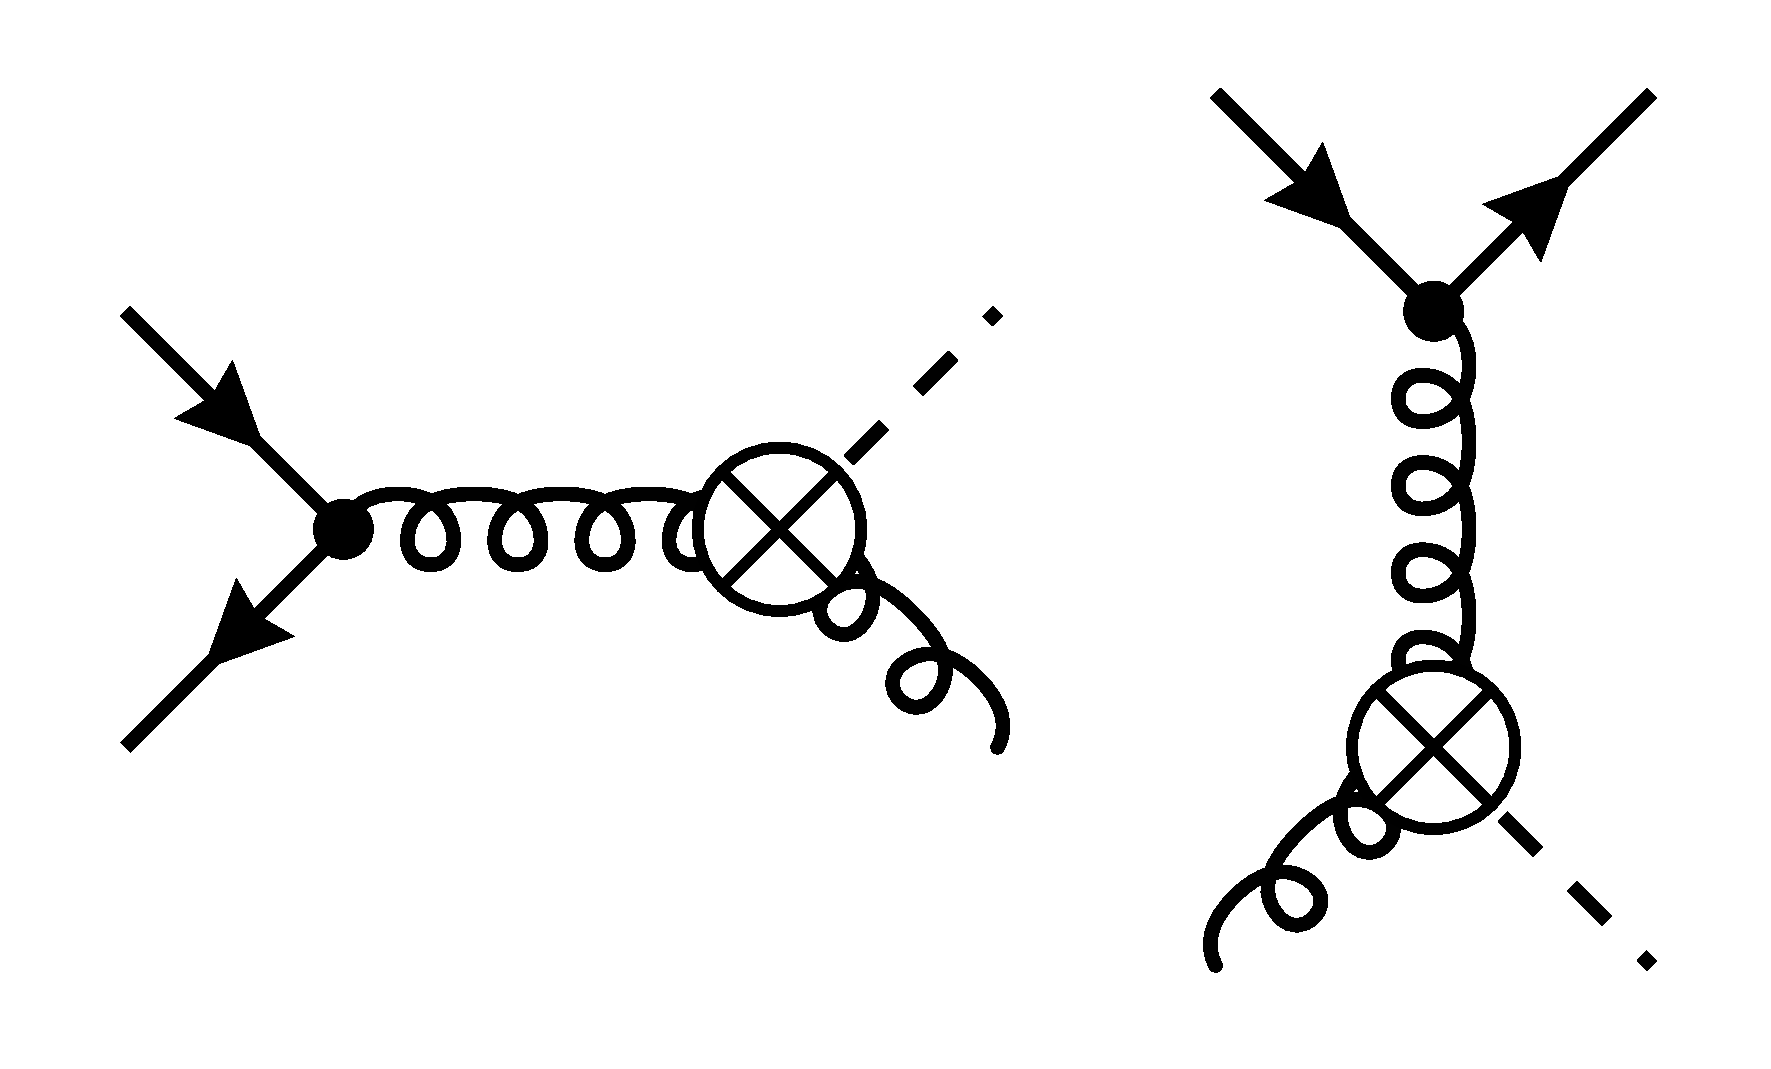
\includegraphics[scale=0.15]{Images/NLO_Feynman_diagrams/qqHg.pdf}
\caption{Feynman diagrams contributing to the $q \bar{q}$ (left) and $q g$ (right) channel of the Higgs production cross section.}
\label{fig:4:qqHg}
\end{figure}
The amplitude for $q \bar{q} \rightarrow H g$ does not exhibit any collinear or soft divergences, rendering collinear renormalization unnecessary. The result for the cross section reads
\begin{equation}
\hat{\sigma}_{q \bar{q} \rightarrow H g} = \frac{1}{486 \pi^2} \frac{\alphas^3}{v^2} \Theta (1 - \xi) \left(1 - \xi \right)^3.
\end{equation}
The $qg$-channel, on the other hand, has a collinear divergence when the final state quark becomes collinear to the initial state quark. After collinear renormalization, we find for the cross section
\begin{equation}
\begin{split}
&\hat{\sigma}_{qg \rightarrow Hg} + \hat{\sigma}_{qg \rightarrow Hg}^C = \frac{\alphas^3}{576 \pi^2 v^2} \Theta (1 - \xi) \\
& \hspace{4cm} \times \bigg \lbrace (1 - \xi) \frac{3 \xi - 7}{3} + \frac{1}{2} \xi P_{gq}(\xi) \left[1 + \log\!\left(\frac{s}{\mu^2} \right) +2 \log\!\left(1 - \xi \right) \right] \bigg \rbrace.
\end{split}
\end{equation}

\begin{figure}[ht]
\centering
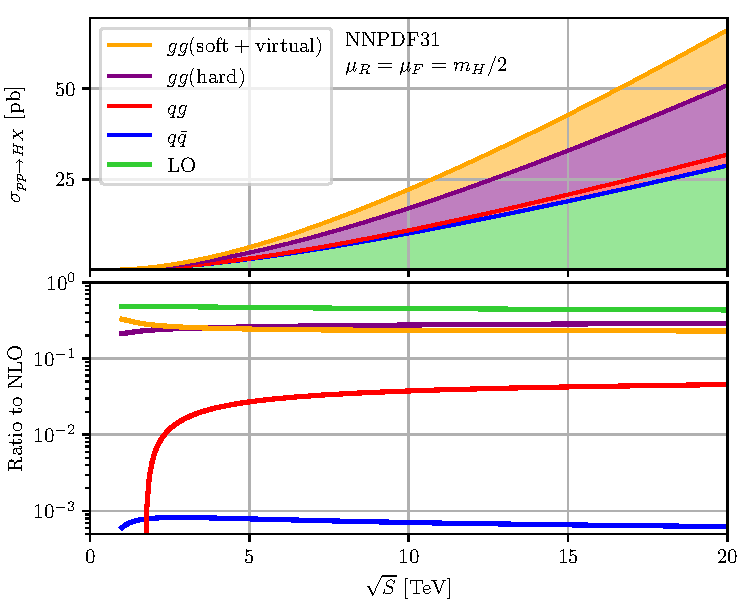
\includegraphics[width=\figurewidth]{Images/channel_comparison_HTL_NLO.pdf}
\caption{Hadronic cross section as a function of the hadronic center-of-mass energy. The total cross section is partitioned into its various channels. The channel denoted \textit{soft + virtual} collects the leading terms of the threshold expansion around $(1 - \xi)$ in Eq.~\eqref{eq:4:ggHX_NLO_HTL_cross_section}, that is all terms proportional to $\delta (1 - \xi)$ and irreducible plus distributions. The lower plot shows the ratio of the various channels to the \acs{NLO} cross section. The computational setup is described in the \hyperref[chap:notation_and_conventions]{Conventions}.}
\label{fig:4:channel_comparison}
\end{figure}
After convolution of the partonic cross section with the partonic luminosity we get the hadronic cross section, which is displayed in Fig.~\ref{fig:4:channel_comparison} as a function of the hadronic center-of-mass energy. The cross section is split into the various channels. The soft + virtual channel denotes all contributions which originate from integrating the delta function $\delta (1 - \xi)$ and irreducible plus distributions, \ie\ terms of the form
\begin{equation}
\left(\frac{f(\xi)}{1 - \xi} \right)_+ \BigO{(1 - \xi)^0}.
\end{equation}
At \acs{NLO}, only gluon-induced Higgs production (see Eq.~\eqref{eq:4:ggHX_NLO_HTL_cross_section}) contributes to the soft + virtual channel.

The majority of the hadronic cross section is due to a gluon-gluon initial state, making up more than 95\% of the total cross section over the full spectrum of energies. Roughly half of this contribution comes from \acs{LO}. The other half is composed, yet again, of roughly two equal parts, the soft + virtual contribution and the remaining real radiation part. The quark-gluon initial state has the second-largest impact, whereas quark-quark induced Higgs production is completely negligible, contributing below 1\textperthousand. The large suppression of the $q\bar{q}$ channel is almost entirely due to the reduced partonic luminosity of the channel. Indeed, from Fig.~\ref{fig:2:luminosity}, we see that the $q \bar{q}$ flux is roughly 30 times smaller than the $q g$ one. This is also the order of magnitude of the ratio of the $qg$ and $q \bar{q}$ induced Higgs production cross section.

The gluon-gluon and quark-gluon luminosities, on the other hand, are rather similar, especially close to the production threshold, where most of the contributions to the cross section originate, as larger values of $\xi$ are suppressed by $\mathcal{L}/\tau$. Yet, we observe that the quark-gluon channel contributes almost an order of magnitude less than in the gluon-gluon channel. To investigate the origin of this suppression, we can look at the coefficient of the logarithm $\log (\mu^2)$ which is predetermined by the \acs{RGE}
\begin{equation}
\frac{\partial \hat{\sigma}_{qg \rightarrow Hq}}{\partial \log \mu^2} = -\frac{\alphas}{2 \pi} \int_0^1 \dd \xi \, P_{gq}(\xi) \hat{\sigma}_{gg \rightarrow H}, \quad \frac{\partial \hat{\sigma}_{gg \rightarrow Hg}}{\partial \log \mu^2} = -2 \times \frac{\alphas}{2 \pi} \int_0^1 \dd \xi \, P_{gg}(\xi) \hat{\sigma}_{gg \rightarrow H}.  \
\end{equation}
At the threshold, the ratio of the logarithmic coefficients of the quark-gluon and the gluon-gluon channel is thus $C_F/(4 C_A) = 1/9$. Incidentally, this is also roughly the ratio we observe between the cross sections of the two channels. The origin of the suppression is thus partly due to the difference in the color factor and the additional combinatorial factors in the gluon-gluon channel.

Since the \acs{NLO} corrections are of the same magnitude as the \acs{LO} cross section, the perturbative result is not yet reliable. One would need to go to even more loops and higher multiplicities in the hope to reach perturbative convergence.

\subsection{Phenomenological Application} \label{subsec:4:phenomenological_application}
Having discussed the \acs{HTL} at length, it is important to investigate how well the approximation works for phenomenological applications. In Fig.~\ref{fig:4:HTL_accuracy}, we show the relative error of the cross section in the \acs{HTL} compared to the results with a finite quark mass for different powers of $\alphas$ in the various partonic channels.

\begin{figure}[ht]
\centering
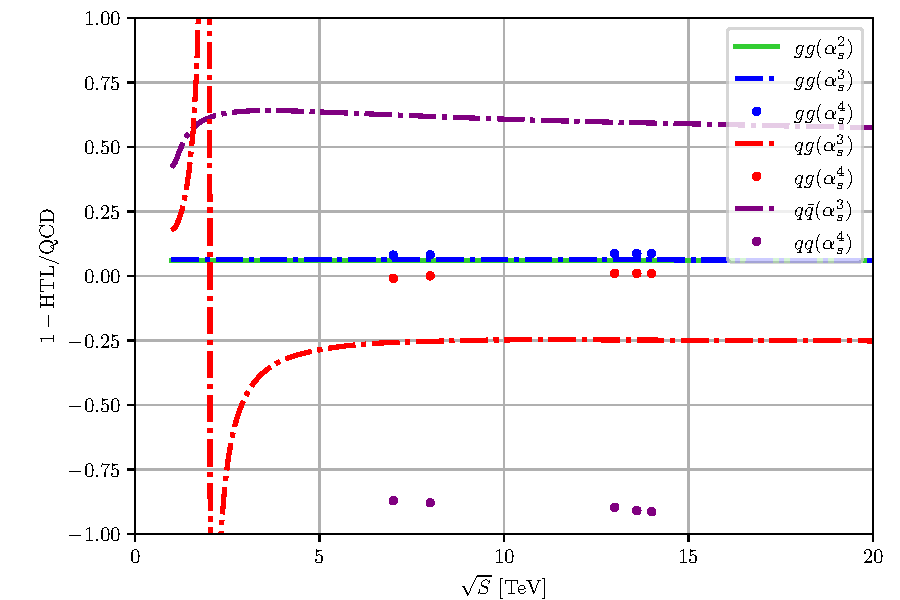
\includegraphics[width=\figurewidth]{Images/HTL_accuracy.pdf}
\caption{Relative error of the \acs{HTL} compared to the results with finite top-quark mass for various center-of-mass energies. Displayed are contributions to the cross section in each partonic channel. The computational setup is described in the \hyperref[chap:notation_and_conventions]{Conventions}. The methods to compute the \acs{NNLO} results with finite top-quark mass are described in Chapter~\ref{chap:5:computational_details}.}
\label{fig:4:HTL_accuracy}
\end{figure}
At \acs{LO}, the \acs{HTL} underestimates the cross section by around $6.5$\%. In the \acs{HTL}, the Higgs-gluon form factor is accurate up to power corrections of order $z = m_H^2/4m_t^2 \approx 13\%$, so the observed accuracy of the approximation aligns with our expectations. For radiative corrections, $m_H^2/m_t^2 \approx 52\%$ is the more natural expansion parameter and the quark-gluon as well as the quark-quark channel show that they are indeed only roughly $50\%$ accurate.

The gluon-gluon channel on the other hand shows a remarkable property: the accuracy of the \acs{HTL} stays quite constant across perturbative orders in $\alphas$. In our opinion, this feed is explained by the fact that much of the structure of the perturbative corrections is dictated by lower orders, and that, for this channel in particular, these kinds of corrections turn out to be numerically large. Indeed, we can apply \textit{Catani's I operator}~\cite{Catani:1996vz} to predict the poles, as well as the overall factor $(-m_H^2/\mu^2)^{-\epsilon}$, of the Higgs-gluon form factor in Eq.~\eqref{eq:4:HTL_formfactor}. So the part of the partonic cross section which is derived from \acs{LO} reads
\begin{equation}
\begin{split}
&\hat{\sigma}_{gg \rightarrow H} \Big \vert_{\propto \sigma_{gg \rightarrow H}^{(0)}} = \frac{\pi}{576 v^2} \xi  \left(\frac{\alphas}{\pi} \right)^2 \delta(1 - \xi) \\
&\qquad \times \left[ \left( 1 + \epsilon + \BigO{\epsilon^2} \right) + \frac{\alphas}{\pi} \left(\frac{m_H^2}{\mu^2} \right)^{-\epsilon} \left(-\frac{3}{\epsilon^2} - \frac{3}{\epsilon} - 3 + \frac{3 \pi^2}{2} + \BigO{\epsilon} \right) + \BigO{\alphas^2} \right].
\end{split}
\label{eq:4:ggH_xSec_propto_LO}
\end{equation}
Numerically, the finite part is largely dominated by the $\pi^2$ term which originated from the analytic continuation of the Sudakov (double) logarithm. The analytic continuation needed at time-like momentum transfer thus causes a large logarithm. The logarithm, on the other hand, stems from a soft-gluon exchange in the loop.

For the real-radiation cross section, we can once again already anticipate the initial-state-collinear as well as the soft divergences
\begin{equation}
  \begin{split}
  & \hat{\sigma}_{gg \rightarrow H g} = \frac{1}{576 \pi^2} \frac{\alphas}{v} \left(1 - \xi \right)^{-1 - 2 \epsilon} \left( \frac{s}{\mu^2} \right)^{-\epsilon} \Theta (1 - \xi) \\
  & \quad \times \left[ - \frac{1}{\epsilon} \xi (1 - \xi) P_{gg}^{(0)}(\xi) \frac{2 (-1 + 2 \epsilon) \Gamma (-\epsilon)}{\Gamma (3 - 2 \epsilon)} +  (1 - \xi)^2 \cdot (\cdots)  \right].
  \end{split}
\end{equation}
The $(1 - \xi)^2$ terms, which we denoted by $(\cdots)$ are finite and regular in the soft limit $\xi \rightarrow 1$. We know that there cannot be any terms of order $(1 - \xi)$ apart from those in the splitting function because every term in the matrix element~\eqref{eq:4:ggHg_Amp} which is constant in the soft limit, still has collinear divergences in the phase-space. \Ie\ all next to soft contributions are captured in the splitting function. In fact, if we compare with the cross section in Eq.~\eqref{eq:4:sigma_ggHg}, then we see that the actual lowest order term is even $(1 - \xi)^4$.

The partonic luminosity together with the factor $1/\tau$ causes a strong enhancement of the phase-space region close to the threshold $\xi \rightarrow 1$ or $\tau \rightarrow m_H^2/S$. Therefore, the hadronic cross section will be well approximated by convolving the inclusive cross section
\begin{equation}
\begin{split}
& \hat{\sigma}_{gg \rightarrow HX} \Big \vert_{\propto \sigma_{gg \rightarrow H}^{(0)}} = \frac{\alphas^2}{576 \pi v^2} \Theta(1 - \xi) \bigg \lbrace \delta(1 - \xi) \\
& \quad + \frac{\alphas}{\pi} \bigg [ \delta(1 - \xi) \pi^2\left( \frac{3}{4} + \BigO{1/\pi^2} \right) + 6 \left( 1 + \xi^4 + (1 - \xi)^4 \right) \left(\frac{\log (1 - \xi)}{1 - \xi} \right)_+ \\
& \hspace{10cm} + \xi P_{gg}(\xi) \log \left(\frac{s}{\mu^2} \right) \bigg ] \bigg \rbrace.
\end{split}
\end{equation}

Numerically, we find that the approximation is around $90\%$ accurate at \acs{NLO}. The main deviations are caused by the soft-virtual channel. We can therefore expect to see deviations in the rescaling factor
\begin{equation}
r^{\mathrm{N}^n\mathrm{LO}} = \frac{\sigma_{pp \rightarrow HX}^{\mathrm{QCD}, \mathrm{N}^n \mathrm{LO}}}{\sigma_{pp \rightarrow HX}^{\mathrm{HTL}, \mathrm{N}^n \mathrm{LO}}}
\end{equation}
across perturbative orders of the order of $10\%\times m_H^2/4m_t^2 \approx 1\%$ based on the gluon-gluon channel alone. The quark-gluon channel contributed only 3\% to the cross section at \acs{NLO}, and the accuracy of the \acs{HTL} is only about 50\% accurate in this channel. In total, we can therefore expect to see deviations in $r^{\mathrm{N}^n\mathrm{LO}}$ of the order of 2\% across perturbative orders.

Strictly speaking, our discussion was limited to \acs{NLO}. However, we claim that most of the arguments are transferable to higher orders in perturbation theory. Indeed, the factor $\pi^2$ we received from analytic continuation of the Sudakov logarithm will also be encountered at higher order, and the effects can be resummed to all orders~\cite{Ahrens:2008qu}. Ergo, the driving contribution is indeed proportional to the born cross section. This procedure is also sometimes referred to as $\pi^2$\textit{-resummation} (see Section~\ref{subsec:4:scale_uncertainties} for more details). At high orders of perturbation theory, it was demonstrated~\cite{Anastasiou:2016cez} that the quality of the resummation deteriorates, meaning that the Sudakov logarithms are no longer the driving contributor to the soft-virtual contribution. We can therefore expect to see larger deviations from the exact rescaling at higher orders of perturbation theory. Similarly, our discussion on how to obtain the leading coefficients of the threshold expansion by requiring cancellation of initial-state collinear divergences can also be transferred to higher orders of perturbation theory~\cite{Anastasiou:2014lda} (see Section~\ref{subsec:4:scale_uncertainties} for more details). This way, at N${}^n$LO, it is in principle possible to correctly predict the first $n$ leading logarithms from lower orders, and the leading logarithm is dictated by the \acs{LO} cross section.

We can exploit the fact that the rescaling parameter only receives small corrections in order to improve the \acs{HTL} cross section results. This works by rescaling the \acs{HTL} results by
\begin{equation}
\sigma_{pp \rightarrow HX}^{\mathrm{rHTL}, \mathrm{N}^n\mathrm{LO}} = r^{\mathrm{LO}} \sigma_{pp \rightarrow HX}^{\mathrm{HTL}, \mathrm{N}^n\mathrm{LO}},
\end{equation}
where the superscript ``\acs{rHTL}'', now refers to the \textit{rescaled heavy top limit}. Since the gluon-gluon channel is the dominant production channel and here the rescaling factor remains quite constant across the perturbative orders, the \acs{rHTL} cross section yields a good approximation ($\sim 2 \%$) for the Higgs production cross section\footnote{Excluding the effects from light quarks and electroweak corrections.}.




\section{Theory Status} \label{sec:4:theory_status}
Having analyzed the gluon-gluon-fusion Higgs production cross section at \acs{LO}, and \acs{NLO} in the \acs{HTL}, we are now equipped with all concepts to discuss state-of-the-art theory predictions.

As already mentioned, the most precise theoretical predictions come from N${}^3$LO cross sections in the \acs{rHTL}~\cite{Anastasiou:2015vya, Anastasiou:2016cez}. They apply the method of reverse unitarity (see section \ref{subsec:2:phase_space_integration}) to perform the phase-space integration fully analytically. The cross section is calculated in terms of a deep expansion in the threshold parameter $(1 - \xi)$
\begin{equation}
\hat{\sigma}_{ij \rightarrow HX} = \delta_{ig} \delta_{jg} \hat{\sigma}_{\mathrm{SV}} + \sum_{n = 0}^N c_{ij}^{(n)} (1 - \xi)^n,
\label{eq:4:threshold_expansion}
\end{equation}
where $\hat{\sigma}_{\mathrm{SV}}$ is the leading term, the soft-virtual contribution we already encountered, which only constitutes $\delta$-functions and plus-distributions. The soft-virtual contribution has been calculated at \NNNLO\ in Ref.~\cite{Anastasiou:2014vaa}. Because the partonic luminosity is concentrated heavily around the threshold region, one would expect to see good convergence of the threshold expansion of the hadronic cross section. Indeed, Ref.~\cite{Anastasiou:2015vya} computed the first 37 terms of the threshold expansion, and found that the hadronic cross section is already well approximated by the first five terms.

In the meantime, results without reliance on the threshold expansion have become available~\cite{Mistlberger:2018etf}, confirming the expected accuracy of the threshold expansion and shifting the total cross section by around $+0.10\ \mathrm{pb}$ at $13\ \TeV$.

In Fig.~\ref{fig:4:energy_scan_rHTL} we show the results for the gluon-gluon-fusion cross section in the \acs{rHTL} at various perturbative orders as a function of the hadronic center-of-mass energy.
\begin{figure}[ht]
\centering
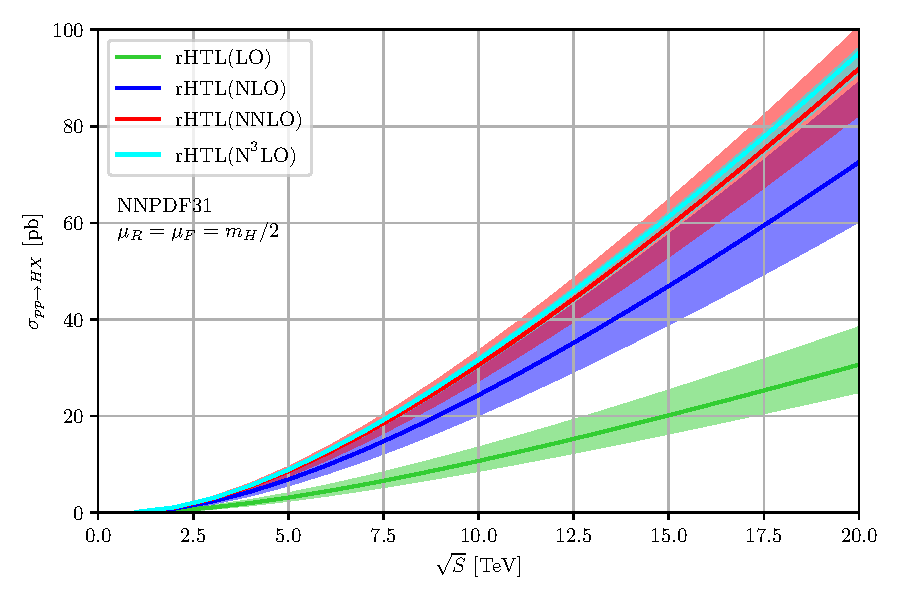
\includegraphics[width=\figurewidth]{Images/energy_scan_HTL.pdf}
\caption{Gluon-gluon-fusion hadronic cross section as a function of the center-of-mass energy. Displayed are results computed in the \acs{rHTL} at various perturbative orders. Transparent bands indicate the scale uncertainty calculated by variation of $\mu_R$ in the range $[m_H/4, m_H]$. The computational setup is described in the \hyperref[chap:notation_and_conventions]{Conventions}. The plot was created with the help of \texttt{SusHi}~\cite{Harlander:2012pb, Harlander:2016hcx}.}
\label{fig:4:energy_scan_rHTL}
\end{figure}

As we discussed before, the \acs{NLO} cross section is about twice as large as predicted in the Born approximation. \acs{NNLO} corrections are still sizeable, contribution roughly $20\%$ to the cross section. The \acs{NLO} scale uncertainties underestimate the effect of higher orders, as the central \acs{NNLO} cross section is outside the previous uncertainty bands. Only when we go to N${}^3$LO do we see perturbative convergence and corrections consistent with the previous scale uncertainty bands. The scale uncertainties at this order are below $4\%$ for the displayed collision energies.

At this level of precision, it becomes important to investigate other sources of uncertainty and perform a careful evaluation of their impact on the cross section. The most important sources are:
\begin{itemize}
  \item The scale uncertainties,
  \item The \acs{PDF} uncertainties,
  \item Uncertainties related to electroweak corrections,
  \item Uncertainties related to finite top-quark masses,
  \item Uncertainties related to light quarks.
\end{itemize}
In the following we will discuss them one-by-one.

\subsection{Scale Uncertainties}\label{subsec:4:scale_uncertainties}
Scale uncertainties serve as an estimate of \acs{MHOU}. They are typically computed by a 7-point scale variation, meaning that the cross section is evaluated at a central scale $\mu$ and the additional 6 points $(\mu_R, \mu_F) = (\mu/2, \mu/2)$, $(\mu/2, \mu)$, $(\mu, \mu/2)$, $(2 \mu, \mu)$, $(\mu, 2 \mu)$, $(2 \mu, 2 \mu)$. The envelope of the cross section at the seven points then forms the scale uncertainty. Since neither the renormalization nor the factorization scale are physical, observables like the cross section are in principle independent of these scales. However, as we are truncating the perturbative series at some fixed order, we are left with some residual scale dependence. The scale dependence is therefore a good indicator of missing higher orders. Even so, at low orders the scale uncertainties cannot always be trusted as Fig.~\ref{fig:4:energy_scan_rHTL} illustrates nicely.

\begin{figure}[ht]
\centering
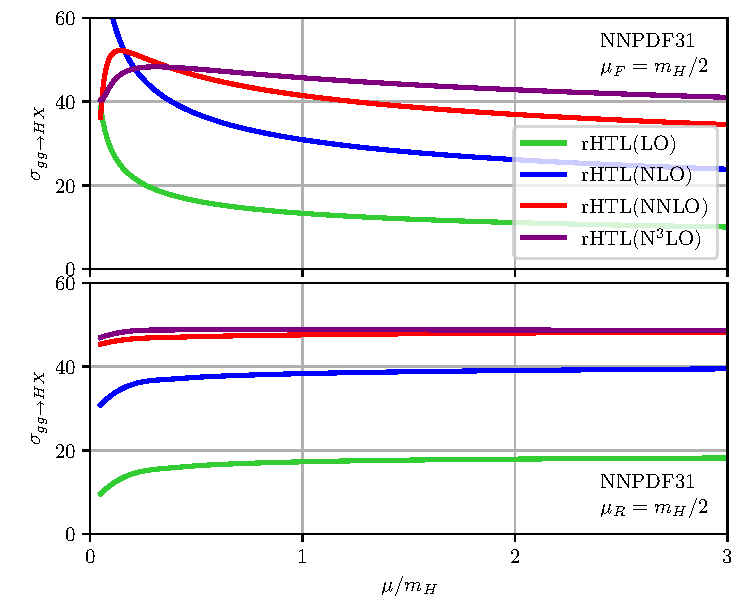
\includegraphics[width=\figurewidth]{Images/scale_scan.pdf}
\caption{Hadronic cross section as a function of the renormalization scale (top panel) and factorization scale (bottom panel). The respective other scale is kept fixed at $m_H/2$. The computational setup is described in the \hyperref[chap:notation_and_conventions]{Conventions}. The plot was created with the help of \texttt{SusHi}~\cite{Harlander:2012pb, Harlander:2016hcx}.}
\label{fig:4:scale_scan}
\end{figure}
Fig.~\ref{fig:4:scale_scan} shows the functional dependence of the hadronic cross section on the renormalization and factorization scale for various perturbative orders. We see that there is very little dependence on the factorization scale, \ie\ the vast majority of the scale uncertainties derive from the variation of renormalization scale. This also justifies why the scale uncertainties in Fig.~\ref{fig:4:energy_scan_rHTL} are computed by only varying the renormalization scale, while the factorization scale was kept fixed at the central value. We also observe that the dependence on the scale nicely stabilizes as we increase the perturbative precision. For the central scale, $\mu_R = \mu_F = m_H/2$ has become the de facto standard for the inclusive cross section and is also the recommendation of the Higgs Working Group~\cite{LHCHiggsCrossSectionWorkingGroup:2016ypw}. The observed functional dependence in Fig.~\ref{fig:4:scale_scan} supports this choice, as the \NNNLO\ corrections are minor at this scale and the cross section is particularly flat in this regime. It should be noted that the minor dependence on the factorization scale is only observed for the total cross section. If instead, we are considering individual production channels, the functional dependence remains very large because the DGLAP equations mix the quark and gluon \acs{PDF}s.

The scale uncertainties can be further reduced by including higher order corrections. Although full N${}^4$LO predictions are still beyond the current state-of-the-art in computational capabilities, we can predict at least some parts of the higher order corrections.

\textbf{Results in the soft-virtual approximation}\\
Since the partonic luminosity is sharply peaked around the threshold (see Fig.~\ref{fig:2:luminosity}), corresponding to $\xi \rightarrow 1$ (or alternatively $\tau \rightarrow m_H^2/S$), we can get a good approximation of the hadronic cross section by expanding the partonic cross section around the threshold as seen in Eq.~\eqref{eq:4:threshold_expansion}. The leading term, \ie\ the soft-virtual approximation has already been computed up to four loops~\cite{Das:2020adl} in the \acs{HTL}.
\begin{table}[ht]
\centering
\begin{tabular}{ccccc}
& $\sigma_\text{rHTL}$ [pb] & $\Delta \sigma_\text{rHTL}$ [pb] & $\Delta \sigma_{\text{s.-v.}}$ [pb] & $\Delta\sigma_{\text{s.-v.}}/\Delta\sigma_\text{rHTL}$ \\
\hline
LO & $16.3$ & $16.3$ & $+16.3$ & 1 \\
NLO & $35.1$ & $18.8$ & $+7.8$ & $0.42$ \\
NNLO & $44.3$ & $9.1$ & $+3.4 \pm 4.8$ & $0.37$ \\
N${}^3$LO & $45.8$ & $1.6$ & $+1.2 \pm 2.2$ & $0.83$ \\
N${}^4$LO &  &  & $+0.14 \pm 0.24$ & \\
\end{tabular}
\caption{Comparison of the cross section computed in the full \acs{rHTL} ($\sigma_\text{rHTL}$) and in the soft-virtual approximation ($\sigma_{\text{s.-v.}}$). $\Delta \sigma_{\text{s.-v.}}$ and $\Delta \sigma_{\text{rHTL}}$ refer to the perturbative correction of the respective order. The assigned uncertainties are computed based on lower oders using $\delta(\Delta  \sigma^{\text{N}^n\text{LO}}_{\text{s.-v.}}) =  \text{max} \lbrace | 1 - \Delta \sigma^{\text{NLO}}_\text{rHTL}/ \Delta \sigma^{\text{NLO}}_{\text{s.-v.}}|,\ldots,  | 1 - \Delta \sigma^{\text{N}^{n-1}\text{LO}}_\text{rHTL}/\Delta \sigma^{\text{N}^{n-1}\text{LO}}_{\text{s.-v.}} | \rbrace \Delta  \sigma^{\text{N}^n\text{LO}}_{\text{s.-v.}}$. Results up to \NNNLO\ have been computed with \texttt{SusHi} using the computational setup described in the \hyperref[chap:notation_and_conventions]{Conventions} at a hadronic center-of-mass energy of 13~TeV. The N${}^4$LO results for the soft-virtual approximation were taken from Ref.~\cite{Das:2020adl}. Note that the authors of that reference use a slightly altered computational setup.}
\label{tab:4:soft_virtual_approximation}
\end{table}
In Tab.~\ref{tab:4:soft_virtual_approximation}, we show a comparison of the cross section in the soft-virtual approximation (rescaled) with the corresponding results in the \acs{rHTL}. We can see that the approximation is only qualitative, meaning that it only captures the rough magnitude of the contribution. We assigned a conservative error of the soft-virtual approximation based on the order at which the approximation works the worst and then rescaled to the respective order. The soft-virtual approximation is therefore not suited for precision predictions, but can give us valuable insides into the order of magnitude of the corrections.

The soft-virtual approximation can be further improved. As we discussed in Section~\ref{subsec:4:phenomenological_application}, the cancellation of initial state collinear divergences can be leveraged to determine the leading logarithms of the cross section. For example at N${}^4$LO, the coefficients of the logarithms\footnote{In fact, one can also get parts of the $\log^4 (1 - \xi)$ coefficient.}
\begin{equation}
\log^{7} (1 - \xi), \log^{6} (1 - \xi), \text{ and } \log^{5} (1 - \xi)
\end{equation}
in $c_{ij}^{(0)}$ can be determined. This is especially important to stabilize the factorization scale dependence since otherwise we would introduce an additional contribution to the cross section which is only present in one of the partonic channels, the gluon-gluon channel.

At the central scale of $\mu_R = \mu_F = m_H/2$, the partial N${}^4$LO contribution shifts the cross section by about $+0.3\%$. Scale uncertainties are reduced from around $4\%$ to below $2\%$. The systematic uncertainty coming from the truncation of the threshold expansion is estimated by comparing the full cross section results with the soft-virtual approximation at lower orders in perturbation theory, and rescaling the error to the N${}^4$LO correction (see Eq.~\eqref{eq:6:SV_error_estimate}). The error is estimated to be around $0.5\%$ of the total cross section.

\textbf{Threshold Resummation}\\
The threshold logarithms appearing in $c_{ij}^{(0)}$ can actually be resummed to all orders. The hadronic cross section can be cast into the form
\begin{equation}
\sigma (N) = \sum_{ij} f_i(N, \mu_F) f_j(N, \mu_F) \hat{\sigma}_{ij}(N, \mu_R, \mu_F),
\end{equation}
where we switched from $\tau$-space to $N$-space by means of a \textit{Mellin transform}
\begin{equation}
\sigma (N) \equiv \int_0^1 \dd \tau \, \tau^{N - 1} \frac{\sigma (\tau)}{\tau}.
\end{equation}
In $N$-space, also called \textit{Mellin space}, the threshold region $\tau \rightarrow m_H^2/S$ corresponds to the limit $N \rightarrow \infty$. In this limit, it can be shown~\cite{Catani:2003zt, Sterman:1986aj, Catani:1989ne, Catani:1990rp} that the partonic cross section satisfies the resummed form
\begin{equation}
\hat{\sigma}_{ij}(N) = \delta_{ig} \delta_{jg} \hat{\sigma}_{gg \rightarrow H}^{\mathrm{LO}} C_{gg} \exp\!\left[ \mathcal{G}_H(\log N) \right] + \BigO{1/N}.
\end{equation}
$C_{gg}$ collects all constant contributions for $N \rightarrow \infty$ and can therefore be extracted from lower orders in the large $N$ limit. $\mathcal{G}_H(\log N)$ contains the threshold logarithms, which get resummed by exponentiation. It requires the cusp anomalous dimension---now known at four-loop accuracy~\cite{vonManteuffel:2020vjv}---making it possible to compute the full \NNNLO\ +\ next-to-next-to-next-to-leading logarithm cross section results. The results\footnote{The authors of that reference use a Pad\'e approximation for the four-loop cusp anomalous dimension, as the full result was still unknown at that point in time. They claim that the approximation is highly accurate.}~\cite{Anastasiou:2016cez} show that at the central scale, the fixed and resummed cross section are nearly identical. This can be interpreted as additional validation of our scale choice. Additionally, it confirms the N${}^4$LO soft virtual approximation, which also found that the corrections at the central scale are very close to zero.

$\mathbf{\pi^2}$\textbf{-Resummation}\\
In Section~\ref{subsec:4:phenomenological_application}, we showed that the soft-virtual contribution to the cross section is dominated by a Sudakov logarithm at time-like momentum transfer. This fact can be exploited to predict numerically large coefficients at higher orders and ultimately can be used to perform an all order resummation, sometimes referred to as $\pi^2$-resummation~\cite{Ahrens:2008qu}.

Since the logarithm stems from a soft-gluon exchange, we can apply techniques from \textit{soft-collinear effective theory} (\acs{SCET})~\cite{Bauer:2001yt, Bauer:2002nz} to map the Higgs-gluon form factor to a Wilson coefficient of \acs{SCET}. In \acs{SCET}, we integrate out all the hard modes so that we can approximate
\begin{equation}
G_{\mu \nu}^a G^{a\, \mu \nu} \longrightarrow C_S(-q^2) \times (-q^2) g_{\mu \nu} \mathcal{A}_{n \perp}^{a \, \mu} \mathcal{A}_{\bar{n}\perp}^{a \, \nu},
\end{equation}
where $\mathcal{A}_{n \perp}^{\mu\, a}$ and $\mathcal{A}_{\bar{n}\perp}^{a \, \nu}$ are effective, gauge invariant operators representing gluons traveling along the light-like directions $n$ and $\bar{n}$ defined by the momenta of the incoming hadrons. $q^2$ is the square of the momentum of the operator and $C_S(Q^2)$ is the Wilson coefficient. The Higgs-gluon form factor in \acs{SCET}, and hence the leading logarithmic contribution to the full Higgs-gluon form factor is then simply given by
\begin{equation}
\mathcal{C}(0) \Big \vert_{\mathrm{SCET}} = C_S (-m_H^2 - i 0^+),
\end{equation}
which we can use to match the Wilson coefficient
\begin{equation}
C_S(Q^2) = 1 + \frac{\alphas}{4 \pi} C_A \left( - \ln^2\!\left(\frac{Q^2}{\mu^2}\right) + \frac{\pi^2}{6} \right).
\end{equation}
The key benefit of working in the \acs{SCET} framework is that we can now apply \acs{RGE} methods. Indeed, the Wilson coefficient satisfies the \acs{RGE}
\begin{equation}
\frac{\dd C_S}{\dd \ln \mu} = \left[ \Gamma^A_{\mathrm{cusp}} \ln \frac{Q^2}{\mu^2} + \gamma^S \right] C_S,
\end{equation}
where $\Gamma^A_{\mathrm{cusp}}$ is the cusp anomalous dimension of Wilson lines with light-like segments in the adjoint representation, and $\gamma_S$ is the anomalous dimension of the operator. The solution of the differential equation therefore automatically yields a resummed expression of the Higgs-gluon form factor. The solution can be written in terms of the recursive equation
\begin{equation}
\begin{gathered}
|C_S(-m_H^2)|^2 = U(m_H^2) |C_S(-m_H^2)|^2,  \\
\text{with} \qquad \ln U(m_H^2) = \frac{\alphas (m_H^2)}{\pi}\frac{C_A \pi^2 }{2} \bigg \lbrace 1 + \frac{\alphas(m_H^2)}{4 \pi} \left[C_A \left(\frac{67}{9} - \frac{\pi^2}{3} \right) - T_F n_l \frac{20}{9} \right] + \BigO{\alphas^2} \bigg \rbrace.
\end{gathered}
\end{equation}
We see that the leading $\pi^2$ term matches our findings in Eq.~\eqref{eq:4:ggH_xSec_propto_LO}.

The resummation drastically improves results at low order of perturbation theory. However, at higher orders, the quality of the resummation deteriorates. This indicates that at these orders the factors of $\pi^2$ are no longer dominant. The procedure should therefore \textbf{not} be used to ``improve'' the \NNNLO\ cross sections.

\subsection{PDF Uncertainties} \label{subsec:4:pdf_uncertainties}
All results presented so far, were computed using \acs{NNLO} \acs{PDF} sets, including all \NNNLO\ cross section results. This creates a mismatch between the hard scattering matrix elements and the \acs{PDF}s, so that the cross sections predictions do not, in fact, have full \NNNLO\ accuracy. The reason for applying \acs{PDF} sets at \acs{NNLO} accuracy is the lack thereof at \NNNLO.

\acs{PDF}s are usually fitted to experimental data and then evolved to the desired scale using the DGLAP equation~\eqref{eq:2:DGLAP}. To achieve \NNNLO\ accuracy, we therefore require
\begin{enumerate}
  \item hard scattering amplitudes the \acs{PDF}s can be matched to,
  \item and the \NNNLO\ splitting functions for the DGLAP evolution.
\end{enumerate}
Regarding the first point, the exact \NNNLO\ coefficient functions for \textit{deep-inelastic scattering} in the massless limit have been known for a long time~\cite{Vermaseren:2005qc, Moch:2004xu, Moch:2007rq, Moch:2008fj, Davies:2016ruz, Blumlein:2022gpp}, whereas massive coefficient functions are only available in approximation frameworks~\cite{Kawamura:2012cr, Laurenti:2024anf}. Furthermore, \NNNLO\ predictions for charged- and neutral-current \textit{Drell-Yan} production are also available, both for the total~\cite{Baglio:2022wzu, Duhr:2020sdp, Duhr:2021vwj} and for differential cross sections~\cite{Chen:2021vtu, Chen:2022lwc}. These processes are especially valuable for the matching of the \acs{PDF}s since they are experimentally very clean.

In Mellin space, the DGLAP equation~\eqref{eq:2:DGLAP} transforms from an integral-differential equation to a mere partial differential equation
\begin{equation}
\frac{\partial f_{H,i}}{\partial \log \mu} = - \gamma_{ij}(N, \alphas(\mu)) f_{H, j}(N, \mu),
\end{equation}
where $\gamma_{ij}(N, \alphas)$ is related to the Mellin transform of the splitting functions
\begin{equation}
\gamma_{ij}(N, \alphas(\mu)) = - \frac{\alphas}{\mu} \int_0^1 \dd x \, x^{N - 1} P_{ij}(x, \alphas (\mu)).
\end{equation}
Much progress has been made in evaluating specific moments of the splitting functions~\cite{Moch:2017uml, Moch:2021qrk, Davies:2016jie, Falcioni:2023tzp, Gehrmann:2023cqm, Falcioni:2023luc, Gehrmann:2023iah}. Additionally, parts of the splitting functions can be predicted through resummation techniques at low Bjorken-$x$, at leading logarithmic~\cite{Jaroszewicz:1982gr} and next-to-leading logarithmic~\cite{Ball:1995vc, Ball:1999sh, Bonvini:2018xvt} accuracy. Very recently, all $1 \rightarrow 2$ splitting amplitudes were computed fully analytical by Mistlberger et al.~\cite{Guan:2024hlf}, these describe the limit of amplitudes in which two of the external partons become collinear. It represents one important ingredient of the splitting kernel.

Although the evolution kernels are not yet fully known, the ingredients we do have can be still be used to at least construct an approximate \NNNLO\ \acs{PDF} set. Results for such \acs{PDF} sets were recently published by the \texttt{MSHT}~\cite{McGowan:2022nag} as well as the \texttt{NNPDF}~\cite{NNPDF:2024nan} collaboration, which were then combined in Ref.~\cite{MSHT:2024tdn}. They use the available data for deep-inelastic scattering and Drell-Yan production to fit the \acs{PDF}s. For the running they use (most of) the known Mellin moments of the splitting kernels and smoothly interpolate between them.

In Fig.~\ref{fig:4:pdf_benchmark} and Tab.~\ref{tab:4:pdf_benchmark}, we compare the gluon-gluon-fusion \acs{rHTL} cross section results at \NNNLO\ computed with different approximate \NNNLO\ \acs{PDF} sets.
\begin{figure}[ht]
  \centering
  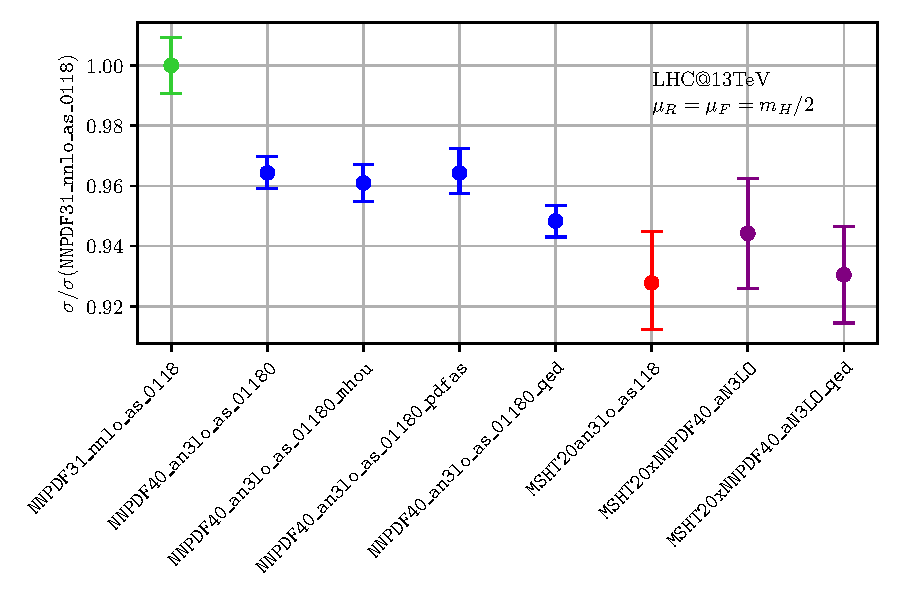
\includegraphics[width=\figurewidth]{Images/pdf_benchmark.pdf}
  \caption{The gluon-gluon-fusion cross section at 13~TeV in the \acs{rHTL} at \NNNLO\ for various \acs{PDF} sets normalized by the cross section computed with the \texttt{NNPDF31\_nnlo\_as\_0118} \acs{PDF} set. The provided uncertainties only include the \acs{PDF} uncertainties. The uncertainty of the normalization is not propagated. The computational setup is described in the \hyperref[chap:notation_and_conventions]{Conventions}. Results were computed using \texttt{iHixs 2}~\cite{Dulat:2018rbf}.}
  \label{fig:4:pdf_benchmark}
\end{figure}
\begin{table}[ht]
  \centering
  \begin{tabular}{l l}
    \hline
    \acs{PDF} & $\sigma_{gg \rightarrow HX}$ [pb] \\
    \hline
    $\mathtt{NNPDF31\_nnlo\_as\_0118}$ & $48.8 \pm 0.46$ \\
    $\mathtt{NNPDF40\_an3lo\_as\_01180}$ & $47.06 \pm 0.26$ \\
    $\mathtt{NNPDF40\_an3lo\_as\_01180\_mhou}$ & $46.90 \pm 0.30$ \\
    $\mathtt{NNPDF40\_an3lo\_as\_01180\_pdfas}$ & $47.06 ^{{+0.40}}_{{-0.33}}$ \\
    $\mathtt{NNPDF40\_an3lo\_as\_01180\_qed}$ & $46.28 \pm 0.26$ \\
    $\mathtt{MSHT20an3lo\_as118}$ & $45.28 ^{{+0.83}}_{{-0.75}}$ \\
    $\mathtt{MSHT20xNNPDF40\_aN3LO}$ & $46.08 \pm 0.89$ \\
    $\mathtt{MSHT20xNNPDF40\_aN3LO\_qed}$ & $45.41 \pm 0.78$ \\
    \hline
  \end{tabular}
  \caption{The gluon-gluon-fusion cross section at 13~TeV in the \acs{rHTL} at \NNNLO\ for various \acs{PDF} sets. The provided uncertainties only include the \acs{PDF} uncertainties. The computational setup is described in the \hyperref[chap:notation_and_conventions]{Conventions}. Results were computed using \texttt{iHixs 2}~\cite{Dulat:2018rbf}.}
  \label{tab:4:pdf_benchmark}
\end{table}
The \texttt{NNPDF40\_an3lo\_as\_01180\_mhou} includes \acs{MHOU}. This encompasses the scale uncertainties of the hard scattering matrix elements the \acs{PDF}s are fitted to, and estimates of the omitted terms in the incomplete \NNNLO\ splitting kernels. In the \texttt{NNPDF40\_an3lo\_as\_01180\_pdfas} \acs{PDF} set, the replicas are created with different values of $\alphas$ between $\alphas (m_Z) = 0.117$ and $0.119$, in order to estimate the $\alphas$ uncertainties. \acs{PDF} sets ending with ``\texttt{\_qed}'', also include corrections from \acs{QED}.

Before the publication of a\NNNLO\ \acs{PDF} sets, the uncertainty due to the mismatch of the \acs{PDF} was often estimated through lower orders rescaled to \NNNLO,
\begin{equation}
\delta (\mathrm{PDF-th}) = \frac{1}{2} \Big \vert \sigma_{gg \rightarrow HX}^{\mathrm{NNLO}, \mathrm{NNLO\ PDF}} - \sigma_{gg \rightarrow HX}^{\mathrm{NNLO}, \mathrm{NLO\ PDF}} \Big \vert .
\end{equation}
This is for example the recommendation of the Higgs Working Group~\cite{LHCHiggsCrossSectionWorkingGroup:2016ypw}. The factor $1/2$ is included as a conservative estimate of the rescaling factor, as the \NNNLO\ effect will be suppressed compared to the \acs{NNLO} one.
For the \texttt{NNPDF31\_nnlo\_as\_0118} \acs{PDF} set at 13~TeV, this uncertainty turns out to be close to $1\%$. However, from Fig.~\ref{fig:4:pdf_benchmark}, we can see that with this approach the impact of the \NNNLO\ \acs{PDF}s is severely underestimated, as the results computed with the a\NNNLO\ \acs{PDF}s is shifted by around $4$-$6\%$. This difference underscores why fully consistent \NNNLO\ \acs{PDF} sets are crucial for accurate cross section predictions.

We can also see that the different approaches followed by the \texttt{NNPDF} and \texttt{MSHT} collaborations, yield central values which are not compatible within the associated uncertainty bands. Furthermore, the \acs{PDF}-uncertainty estimates themselves differ significantly by about a factor of three.

Provided that the \acs{MHOU} are well estimated by the \texttt{NNPDF} collaboration, the approximations of the splitting kernels by a finite number of Mellin-moments seems to be highly accurate, effecting the cross sections only on the level of 1\textperthousand.

The $\alphas$-uncertainties, make up about half of the total \acs{PDF} uncertainty, as visible from the error increase between the \texttt{NNPDF40\_an3lo\_as\_01180} and \texttt{NNPDF40\_an3lo\_as\_01180\_pdfas} \acs{PDF} set.

The inclusion of \acs{QED} effects shifts the cross section by around $-0.6\ \mathrm{pb}$ at $13\ \mathrm{TeV}$.

Because of the sizeable difference between the \acs{PDF}s of the two collaboration we advise using the combined \acs{PDF} sets until the origin of the discrepancy has been identified or full \NNNLO\ \acs{PDF} sets become available.

\subsection{Electroweak Corrections}
Besides the discussed \acs{QCD} corrections, we can also consider electroweak corrections. These are generally suppressed because of the smaller coupling constant $\alpha (m_Z) \approx 1/127$, but the percentage-level precision of our predictions makes an investigation of electroweak effects indispensable.

The electroweak corrections to the \acs{LO} \acs{QCD} partonic cross section can be classified into two categories: the light-quark contributions and the top-quark contributions.
\begin{figure}[ht]
  \centering
  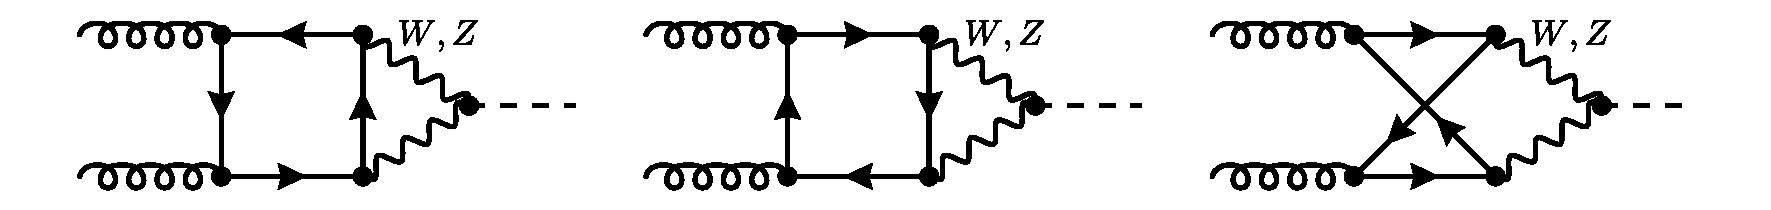
\includegraphics[width=\textwidth]{Images/electro_weak_light.pdf}
  \caption{Light-quark contribution to the \acs{LO} electroweak corrections of the gluon-gluon-fusion Higgs production cross section.}
  \label{fig:4:ew_lq}
\end{figure}
\begin{figure}[ht]
  \centering
  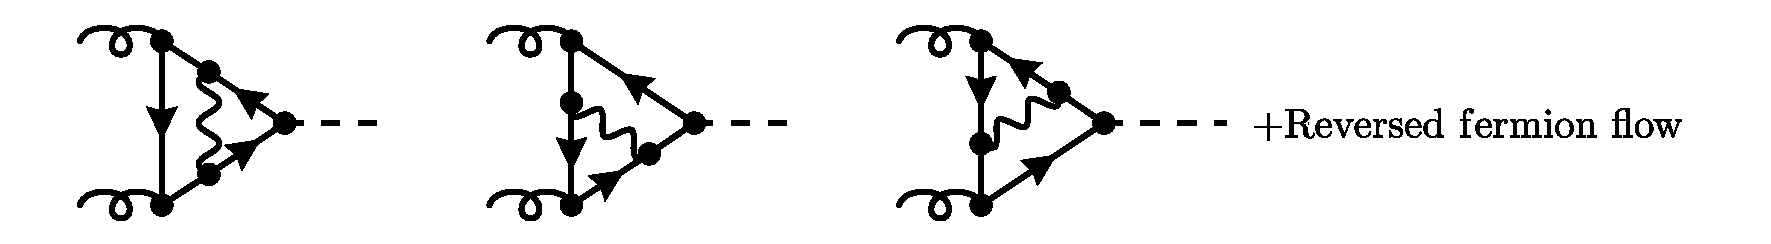
\includegraphics[width=\textwidth]{Images/electro_weak_top.pdf}
  \caption{Top-quark contribution to the \acs{LO} electroweak corrections of the gluon-gluon-fusion Higgs production cross section. The wavy line represents all electroweak gauge bosons ($\gamma, W, Z$).}
  \label{fig:4:ew_top}
\end{figure}
The top-quark contribution contains a Yukawa-coupling of the top, and the light-quark contributions contain all the remaining diagrams. The respective diagrams are depicted in Fig.~\ref{fig:4:ew_lq} and\ \ref{fig:4:ew_top}. Real radiative electroweak corrections like those depicted in Fig.~\ref{fig:4:ew_real} do not contribute to the cross section, since two diagrams which only differ by the direction of the fermion flow exactly cancel. Even though the preconditions are not strictly met, this can be shown analogous to \textit{Furry's theorem}\footnote{Furry's theorem states that the abelian part of the sum of two diagrams that differ only by the direction of a closed fermion vanishes, if there are an odd number of vertices proportional to the $\gamma$-matrices. In the present case, the color factor is $\delta^{c_1 c_2}$, \ie\ it is fully abelian. There is an even number of vertices, however one of the vertices is a Yukawa interaction and hence does not introduce a $\gamma$-matrix. It is easy to show that with these conditions, Furry's theorem still applies.}.
\begin{figure}[ht]
  \centering
  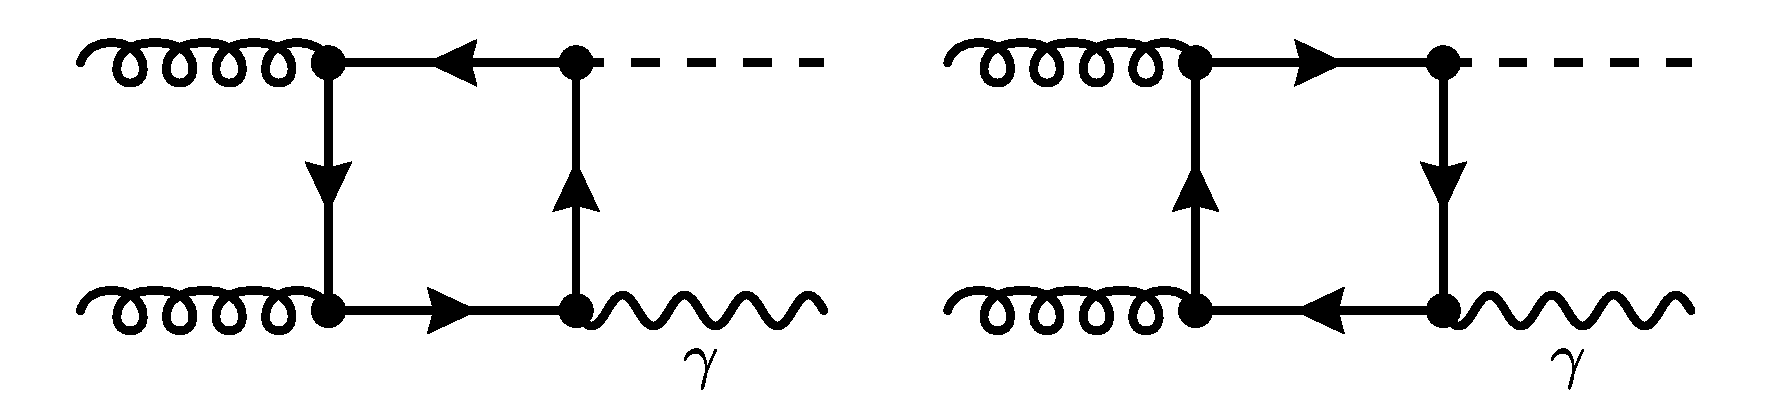
\includegraphics[scale=0.32]{Images/electro_weak_real.pdf}
  \caption{Example Feynman diagrams of radiative electroweak corrections to the gluon-gluon-fusion Higgs production cross section. The remaining four Feynman diagrams can be obtained by permutation of external gluon, photon and Higgs. Two diagrams which differ only by the direction of the fermion flow exactly cancel.}
  \label{fig:4:ew_real}
\end{figure}

The two-loop light-quark contribution to the Higgs-gluon form factor was calculated in Ref.~\cite{Aglietti:2004nj}. The top-quark contribution was then worked out in Refs.~\cite{Degrassi:2004mx, Actis:2008ts, Actis:2008ug}. The latter reference also includes the effect from finite bottom-quark masses, including diagrams in which we encounter flavor changes due to a $W$-boson exchange. The leading electroweak corrections increase the \acs{LO} cross section by around $5\%$. Almost the entirety of this correction is due to the light-quark contribution.

Beyond \acs{LO} in $\alphas$, the hadronic cross section was first estimated at $\BigO{\alphas^3 \alpha}$ using the \acs{HTL} and also treating the massive vector bosons as infinitely heavy~\cite{Anastasiou:2008tj}. Furthermore, since the top-quark contribution was negligible at \acs{LO}, the authors only considered light-quark contribution to the cross section. With this approximation, the electroweak corrections can be incorporated through a modification of the Wilson coefficient
\begin{equation}
\begin{split}
  C_1 = &\left[\frac{\alphas}{4 \pi} C_1^{(0)} + \left(\frac{\alphas}{4 \pi} \right)^2  C_1^{(1)} + \BigO{\alphas^3} \right] \\
  & \quad + \frac{\alpha}{4 \pi} \left[ \frac{\alphas}{4 \pi} C_{1,w}^{(0)} +  \left(\frac{\alphas}{4 \pi} \right)^2  C_{1,w}^{(1)} + \BigO{\alphas^3} \right].
\end{split}
\label{eq:4:ew_Wilson}
\end{equation}
One then finds for the electroweak coefficient
\begin{equation}
  \begin{split}
  &C_{1,w}^{(0)} = -  \frac{2}{\sin^2 \theta_W \cos^2 \theta_W} \left[ \frac{5}{4} - \frac{7}{3} \sin^2 \theta_W + \frac{22}{9} \sin^4 \theta_W \right] - \frac{4}{\sin^2 \theta_W}, \\
  &C_{1,w}^{(1)} = C_{1,w}^{(0)} \frac{14}{3}.
  \end{split}
\end{equation}

The same contribution was later reevaluated in the limit of massless electroweak gauge bosons~\cite{Anastasiou:2018adr} as well as in the soft-gluon approximation~\cite{Bonetti:2018ukf}. Although the approximations make completely different assumptions about the mass spectrum, the phenomenological results turn out to be quite similar, increasing the \acs{NLO} cross section between $5.4$ and $5.2\%$. This shows that the cross section is not very sensitive to the mass of the vector bosons.

Still, results with finite vector-boson masses would be highly desirable and were recently provided by Ref.~\cite{Becchetti:2020wof}. The authors found that the electroweak corrections increase the \acs{NLO} cross section by around $5.1\%$, confirming that the previous approximations were indeed accurate. The $\BigO{\alphas^3 \alpha^2}$ QCD predictions are rescaled to order $\BigO{\alphas^5 \alpha^2}$ using the \acs{rHTL} with electroweak corrected Wilson coefficients (see Eq.~\eqref{eq:4:ew_Wilson}). The electroweak corrections increase the \NNNLO\ \acs{rHTL} cross section by $4.6 \pm 0.6\%$. By far, the dominating source of uncertainty of this contribution is the missing higher order uncertainty. Uncertainties related to the omission of the top-quark contribution, finite quark-mass effects, or partonic channels at $\BigO{\alphas^3 \alpha^2}$ are all below $0.1\%$.

\subsection{Finite Top-Quark Mass Effects}
So far our discussion of perturbative corrections was mainly focused on the \acs{HTL} approximation. In Section~\ref{subsec:4:phenomenological_application}, we explained how the approximation can be improved to also encompass some finite top-quark mass effects by means of rescaling the cross sections. We argued that in the dominant gluon-gluon channel especially, the \acs{rHTL} approximation will be highly accurate. Nevertheless, we also saw significant deviations---in particular for the other partonic channels---which could yield important corrections to the \acs{rHTL} cross section.

This makes the higher-order corrections with finite top-quark mass indispensable. The \acs{LO} calculation with finite top-quark masses presented in Section~\ref{sec:4:LO_xSec} was extended to \acs{NLO} in Refs.~\cite{Djouadi:1991tka, Graudenz:1992pv}. Later, power corrections to the \acs{HTL} of the form $\BigO{m_H^4/m_t^4}$ became available at \acs{NNLO}~\cite{Harlander:2009mq, Harlander:2009my, Pak:2009dg}. Still, a residual theoretical uncertainty of about $1\%$ of the total cross section persisted. Only with the computation of the exact top-quark mass dependence of the \acs{NNLO} cross Section~\cite{Czakon:2021yub} was the uncertainty finally (effectively) eliminated.
\begin{table*}[t!]

\centering
\begin{tabular}{c|r|rr|c}
\hline
\rule{0pt}{1em}
\multirow{2}{*}{channel} & \multicolumn{1}{c|}{$\sigma^\mathrm{NNLO}_\mathrm{rHTL}$ [pb]} &
\multicolumn{2}{c|}{$(\sigma^\mathrm{NNLO}_t-
\sigma^\mathrm{NNLO}_\mathrm{rHTL})$ [pb]} &
$(\sigma^\mathrm{NNLO}_t- \sigma^\mathrm{NNLO}_{1/m_t})$ [pb] \\
& $\BigO{\alphas^2}+\BigO{\alphas^3}+\BigO{\alphas^4}$ & \multicolumn{1}{r}{$\BigO{\alphas^3}$} & \multicolumn{1}{r|}{$\BigO{\alphas^4}$} & $\BigO{\alphas^4}$ \\
\hline
\multicolumn{5}{c}{\rule{0pt}{1em}$\sqrt{S} = 8$\,TeV}\\\hline
$gg$ & $7.39 + 8.58 + 3.88$ &  $+0.0353$ & $+0.0879$ & $-0.047$ \\
$qg$ & $0.55 + 0.26$ & $-0.1397$ & $-0.0153$ & $+0.001 $\\
$qq$ & $0.01 + 0.04$ & $+0.0171$ & $-0.0191$ & - \\\hline
total & $7.39 + 9.14 + 4.18$ &  $-0.0873$ & $+0.0535$ & $-0.046$ \\
\hline
\multicolumn{5}{c}{\rule{0pt}{1em}$\sqrt{S} = 13$\,TeV}\\\hline
$gg$ & $16.30 + 19.64 + 8.76$ & $+0.0345$ & $+0.2431$ & $-0.145$ \\
$qg$ & $1.49 + 0.84$ & $-0.3696$ & $-0.0408$ & $+0.015$ \\
$qq$ & $0.02 + 0.10$ & $+0.0322$ & $-0.0501$ & - \\\hline
total & $16.30 + 21.15 + 9.70$ & $-0.3029$ & $+0.1522$ & $-0.130$ \\
\hline
\end{tabular}
\caption{Comparison of cross sections computed in the \acs{rHTL} ($\sigma_\mathrm{rHTL}$), the cross section with finite top-quark masses ($\sigma_{t}$), and the cross section computed with power corrections ($\sigma_{1/m_t}$) at \acs{NNLO}. The computational setup is described in the \hyperref[chap:notation_and_conventions]{Conventions}. Exact results were extracted from Ref.~\cite{Czakon:2021yub}. The power corrections were computed using \texttt{iHixs 2}~\cite{Dulat:2018rbf}. The quark-quark channel is not yet available with power corrections, which is why we do not include it in the above table. The channel is suppressed by the \acs{PDF}s, \ie\ the total cross section will be left almost unaffected.} \label{tab:4:finite_top_quark_mass_effects}
\end{table*}

The main results of that reference are displayed in Tab.~\ref{tab:4:finite_top_quark_mass_effects} (also see Fig.~\ref{fig:4:HTL_accuracy}). We also compare the cross sections with exact top-quark mass dependence with the $m_H/m_t$ expansion. We see that the finite-top-quark-mass effects are small ($<0.4\%$). In the gluon-gluon channel, the \acs{rHTL} works exceptionally well, approximating the \acs{NNLO} cross section with percent-level accuracy. Again we expect this kind of accuracy on the basis of the rescaling procedure. In the other partonic channels the approximation works significantly worse, showing deviations of up to $19\%$. The sheer dominance of the gluon-gluon channel assures that the total cross section is approximated well by the \acs{rHTL}.

The power corrections $\BigO{m_H^4/m_t^4}$ to the \acs{HTL} do not significantly improve the \acs{rHTL}, but they do get the order of magnitude as well as the sign right.

The residual theoretical uncertainty of the finite-top-quark-mass effects can be estimated from the scale uncertainty of the difference $\sigma_{t} - \sigma_{\mathrm{rHTL}}$, taking into account all correlations.

Since the perturbative series of the cross section is truncated at some fixed order, it will have some residual renormalization scheme dependence. The scheme-dependence of the cross section was investigated in Refs.~\cite{Anastasiou:2016cez, Czakon:2024ywb} including our own analysis. The difference between the on-shell and \MS\ scheme was found to be less than $1$\textperthousand\ of the total cross section, rendering also the uncertainty on the scheme dependence completely negligible.

\subsection{Effect of Light Quarks} \label{subsec:4:effect_of_light_quarks}
In Section~\ref{sec:4:LO_xSec}, we investigated to what extent light quarks affect the gluon-gluon-fusion Higgs production cross section at \acs{LO}. Here, we found that the main contribution arises from the interference with top-quark induced Higgs production. The inclusion of the bottom-quark lowered the cross section by around $6.5\%$ at $13\ \mathrm{TeV}$. The next-heaviest quark---the charm---further reduced the cross section, this time by $1\%$.

Since perturbative corrections are typically quite large in gluon-gluon fusion, it is once again vital to also compute higher-order corrections to the interference. The \acs{NLO} cross section for arbitrary quark masses was computed in Ref.~\cite{Graudenz:1992pv}.

Once again, we estimate the theoretical uncertainty from missing higher orders through the assigned scale uncertainties. The HWG, instead suggests estimating the uncertainty based on lower orders and rescale them to the \NNNLO\ correction in the \acs{rHTL}. Since the light-quark-mass effects are not expected to scale with the cross section of the \acs{rHTL}, we do not believe that this is a reliable estimate of the uncertainty and do not apply them going forward.

\begin{figure}[ht]
  \centering
  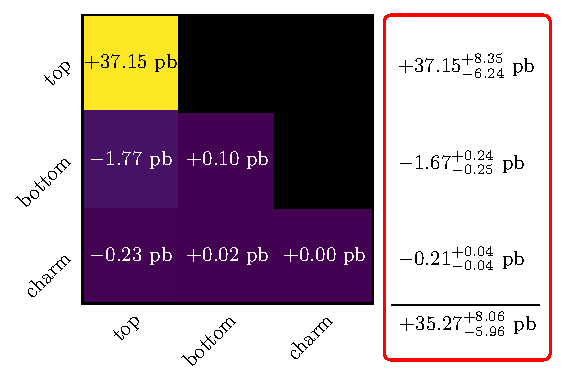
\includegraphics[scale=0.9]{Images/quark_effects_NLO.pdf}
  \caption{$\sigma_{i}$ (diagonals) and $\sigma_{i \times j}$ (off-diagonals) at \acs{NLO} for the three heaviest quark flavors at a hadronic center-of-mass energy of 13 TeV. The red box indicates the sum of each row, and hence the combined effects of each additional flavor. The computational setup is described in the \hyperref[chap:notation_and_conventions]{Conventions}. We use the on-shell scheme for the top-quark mass and the \MS\ scheme for the charm- and bottom-quark masses. The scale uncertainties are computed using 7-point variation.}
  \label{fig:4:quark_effects_NLO}
\end{figure}
The \acs{NLO} results for the pure-flavor and the interference effects are displayed in Fig.~\ref{fig:4:quark_effects_NLO}. We see that the top-bottom interference contribution to the cross section increased in magnitude by $58\%$ from \acs{LO} to \acs{NLO}. We once again observe that the top-bottom interference contribution is by far the most significant one among the effects of light quarks. All other light-quark mass effects are still within the scale uncertainty of the top-bottom interference contribution. Improving these contributions beyond \acs{NLO} is therefore completely unnecessary. Interestingly, we observe that the scale uncertainties of the pure-top and the top-bottom interference contribution are almost perfectly anti-correlated.

With the scale uncertainty, we estimate that effects of missing higher orders in the light-quark contribution are of the order of $7$\textperthousand. However, this estimate is too na\"ive. Indeed, if we choose a different renormalization scheme for the bottom-quark mass, say the \acs{OS} scheme, the top-bottom interference contribution at \acs{NLO} becomes (again at $\sqrt{S} = 13\ \mathrm{TeV}$)
\begin{equation}
\sigma_{t \times b} = -2.42^{+0.19}_{-0.12}\ \mathrm{pb},
\end{equation}
which differs from our previous \MS\ renormalized cross section contribution by $-0.66\ \mathrm{pb}$ or $38\%$. The large discrepancy between the results is somewhat expected since the hard scattering amplitude in the high energy limit roughly scales with $m_b^2$ (see Eq.~\eqref{eq:4:C0_HEL}) and the relation between the on-shell and the \MS\ bottom-mass converges very poorly~\cite{Marquard:2015qpa, Marquard:2016vmy}. Therefore, the cross section can only show a good perturbative convergence in one of the schemes if at all. At \acs{NLO}, we have not determined enough coefficients of the perturbation series to make a reliable argument about the convergence, making higher order predictions indispensable. If we assign the error in a way to encompass both the on-shell- and \MS-renormalized results, it will constitute a $1.7\%$ uncertainty on the total cross section, making it one of the leading sources of uncertainty.

Eliminating this source of uncertainty by computing higher order corrections to the top-bottom interference contribution is one of the major aims of this PhD thesis. With these predictions we want to investigate the perturbative convergence in the different mass-renormalization schemes in order to assess which one works best for phenomenological applications.

The cross sections presented in this section were all computed in the 5\acs{FS}, \ie\ the bottom- and charm-quark were considered massless and could appear in the initial state. Since the hard scattering matrix element vanishes for massless particles, we then proceeded to set the light-quark masses to non-vanishing values in all closed quark loops which couple to the Higgs\footnote{We will later show that this method indeed ensures gauge-invariant \acs{IR}-safe cross sections.}. This ad hoc introduction of quark masses has become the de facto standard for light-quark mass effects in gluon-gluon fusion, but well-grounded justifications of this procedure have been lacking so far. In this PhD thesis, we aim to close this gap and explore the validity of this massification procedure by comparing the results of top-bottom-interference contributions to the same but computed in the 4\acs{FS}, in which the quark-masses are treated consistently.

\subsection{Differential Cross Sections} \label{subsec:4:differential_cross_sections}
Up to this point the main focus of our discussion has been the total cross section of the gluon-gluon-fusion channel. However, differential cross sections can shine some light on the production kinematics of the Higgs and additionally offer a plethora of rich phenomenology and experimental applications. In this section, we will briefly summarize the current status on differential cross sections of Higgs production in the gluon-gluon-fusion channel. The possibilities to study the Higgs production cross section in terms of its kinematics are endless, so our discussion is by no means complete, instead we will focus on the most phenomenologically relevant distributions.

\textbf{The Higgs-$\mathbf{p}_\mathrm{T}$ Distribution}\\
Arguably the most important distribution is the Higgs-$p_T$ distribution
\begin{equation}
\frac{\dd \sigma_{pp \rightarrow HX}}{\dd  p_T},
\end{equation}
where $p_T$ is the transverse momentum of the Higgs with respect to the beam axis. $p_T$-distributions have been calculated up to third order in perturbation theory using the \acs{rHTL}~\cite{Chen:2014gva,Becker:2020rjp}, including subsequent decays to photons~\cite{Chen:2021isd} and leptons~\cite{Chen:2019zel}. The \acs{rHTL} only provides a good approximation of the cross section up to $p_T \sim m_H$ since above this threshold, the top-quark running in the loop is getting resolved. For larger $p_T$, the partonic $p_T$-distribution is well described by a power law. This can be understood with a simple dimensional analysis. Indeed, at large $p_T$, the transverse momentum is the dominant scale, and we can neglect the top-quark mass. In order to match the mass dimension, $-3$, of the differential partonic cross section $\dd \sigma_{pp \rightarrow HX}/\dd p_T$, we require the scaling behavior
\begin{equation}
\frac{\dd \hat{\sigma}_{ij \rightarrow HX}}{\dd p_T} \sim  p_T^{-3}.
\end{equation}
In the \acs{rHTL} on the other hand, the coupling constant is proportional to $1/v^2$ and hence has a non-vanishing mass dimension. The large $p_T$ scaling of the partonic cross section is therefore
\begin{equation}
\frac{\dd \hat{\sigma}_{ij \rightarrow HX}^\mathrm{rHTL}}{\dd p_T} \sim v^{-2}p_T^{-1}.
\end{equation}
Unfortunately, these power-laws no longer hold on the hadronic level because of the convolution with the partonic luminosities. However, since the partonic luminosity dies off extremely quickly, especially at larger values of $\tau$ (see Fig.~\ref{fig:2:luminosity}), the largest contribution to the hadronic cross section will come from the region close to the threshold production. We can then expand the partonic cross section around the threshold yielding
\begin{equation}
\begin{split}
\frac{\dd \sigma_{pp \rightarrow HX}}{\dd p_T} &= \int_{s_\text{min}/S}^1 \frac{\dd \tau}{ \tau} \sum_{ij} \mathcal{L}_{ij}(\tau) \frac{\dd \hat{\sigma}_{ij \rightarrow HX} (\tau S)}{\dd p_T} \\
&\approx \sum_{ij} \frac{\dd \hat{\sigma}_{ij \rightarrow HX} (s_\text{min}) }{\dd p_T} \int_{s_\text{min}/S}^1 \frac{\dd \tau}{\tau} \mathcal{L}_{ij}(\tau),
\end{split}
\end{equation}
where $s_\text{min}$ denotes the minimum partonic center-of-mass energy
\begin{equation}
s_\text{min} = \left(p_T + \sqrt{p_T^2 + m_H^2} \right)^2 \stackrel{m_H \ll p_T}{\approx} 4 p_T^2.
\label{eq:4:smin}
\end{equation}
In good approximation, the ratio of the hadronic cross sections in the \acs{rHTL} and the exact theory must therefore satisfy
\begin{equation}
\frac{\dd \sigma_{pp \rightarrow HX}^{\mathrm{rHTL}}}{\dd p_T} \bigg / \frac{\dd \sigma_{pp \rightarrow HX}}{ p_T} \sim p_T^2/v^2
\label{eq:4:dSig_rHTL/dSig}
\end{equation}
at $p_T \gg m_H$. The inclusion of finite top-quark mass effects is therefore of immense importance especially at large $p_T$ and has been studied up to \acs{NNLO} in Refs.~\cite{Grazzini:2013mca, Buschmann:2014sia, Jones:2018hbb}.

At smaller transverse momentum, $p_T \sim m_H/2$, we can resolve the effects of the lighter quark masses. This is particularly interesting because it demonstrates that this region is sensitive to the Yukawa coupling of the light quarks~\cite{Bishara:2016jga, Bonner:2016sdg}. In a recent study by the \texttt{CMS} collaboration~\cite{CMS:2018gwt}, the authors fitted experimental data to the Higgs-$p_T$ spectrum and were able indirectly determine the following constraints on the coupling modifiers:
\begin{equation}
-1.2 < \kappa_b < 1.1, \qquad -4.9 < \kappa_c < 4.8.
\end{equation}
The effect of light-quark masses on the Higgs-$p_T$ spectrum has been studied up to \acs{NNLO} in Refs.~\cite{Lindert:2017pky, Caola:2018zye, Bonciani:2022jmb,Czakon:2024ywb}.

At \acs{LO} and in all virtual corrections, the Higgs is produced with vanishing $p_T$ because there is no other final state particle for the Higgs to recoil against. The \acs{LO} and all virtual corrections will therefore only contribute to the zero-bin of the distribution. The transverse momentum hence acts as a slicing parameter. Consequently, at small transverse momentum, the cross section will receive large logarithmic enhancements because the cut-off threshold acts an \acs{IR} regulator. These logarithms cancel in the exact cross section, but because the perturbation series is truncated, fixed order results still suffer from their appearance and yield inaccurate results whenever these logarithms become dominant. To stabilize the behavior in these phase-space regions, the logarithms can be resummed to all orders~\cite{Mantler:2012bj,Grazzini:2013mca, Hamilton:2015nsa, Bagnaschi:2015qta, Bagnaschi:2015bop, Frederix:2016cnl, Caola:2016upw, Niggetiedt:2024nmp}.

\textbf{The Higgs-Rapdity Distribution} \\
The Higgs rapidity is defined as
\begin{equation}
\eta_H \equiv \frac{1}{2} \ln \frac{p^0_H + p^3_H}{p^0_H - p^3_H},
\end{equation}
where $p_H$ is the momentum of the Higgs, and the $z$-axis aligns with the beam direction. For the Higgs-rapidity distribtuion all channels, be it real or virtual, can contribute to any bin of the distribution. Consequently, the respective distribution will not show any logarithmic enhancements that require resummation, unlike in the $p_T$-distribution.

The Higgs-rapidity distribution has been calculated up to \NNNLO\ in the \acs{HTL}~\cite{Dulat:2018bfe, Dulat:2017prg}. The effect of finite top-quark masses has been studied at \acs{NNLO} in Ref.~\cite{Niggetiedt:2024nmp}. The effect of finite bottom-quark masses, on the other hand, was recently presented by us~\cite{Czakon:2024ywb} and will be discussed in this PhD thesis.

\subsection{Summary}
The theory uncertainties of the fully inclusive gluon-gluon-fusion Higgs production cross section are summarized in Fig.~\ref{fig:4:error_budget}. The errors on the various sources of uncertainty are assigned according to the above description (for details see Section~\ref{sec:6:recommendations}). The uncertainty on the top-bottom interference contribution is assigned based on the difference between the \acs{NLO} cross sections with an \acs{OS} and \MS\ renormalized bottom-quark mass.
\begin{figure}[ht]
\centering
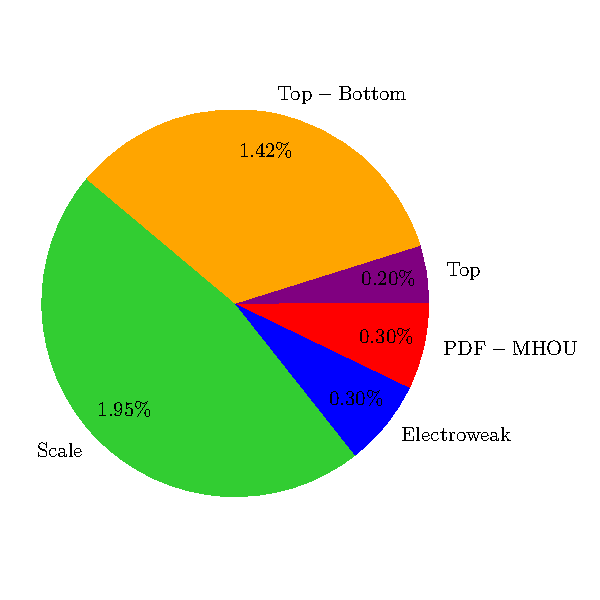
\includegraphics[scale=0.8]{Images/error_budget_before.pdf}
\caption{Total error budget of the fully inclusive gluon-gluon-fusion Higgs production cross section at 13\ TeV. The errors on the various sources of uncertainty are estimated as described in Section~\ref{sec:6:recommendations}. For the top-bottom interference contribution, the error is estimated based on the difference between \acs{NLO} cross section with \acs{OS} and \MS-renormalized bottom-quark mass. For asymmetric uncertainty, we use the total span divided by two.}
\label{fig:4:error_budget}
\end{figure}
The main source of uncertainty is the scale uncertainty, which still makes up almost 42\% of the total error budget. The second most dominant source of uncertainty comes from the top-bottom interference contribution which makes up for about a third of the total error. The only other notable error comes from the soft-virtual approximation. Other sources of uncertainty are already reduced to a point where further improvements would no longer affect the total error significantly.

In order to significantly improve the uncertainty of the cross section, one can either refine the scale uncertainties, or the top-bottom interference contribution. The former is very challenging, as one would need to go to five-loop order. In the foreseeable future, this kind of computation seems out of reach. This leaves us only with the second option of improving the uncertainty of the top-bottom interference contribution, by performing the full \acs{NNLO} cross section calculation with finite bottom-quark masses. This shall be the focus of this PhD thesis.